\documentclass[english, 11pt]{article}
% \usepackage[T1]{fontenc}
% \usepackage[latin9]{inputenc}
\usepackage[top = 2cm, left = 2.5cm, right = 2.5cm, bottom = 2cm]{geometry}
\usepackage{enumitem}
% \usepackage{fontspec}
\usepackage{amsmath}
\usepackage{amsfonts}
\usepackage{hyperref}
\usepackage{amstext}
\usepackage{mdframed}
\usepackage{graphicx}
\usepackage{wrapfig}
\usepackage{caption}
\usepackage{multicol}

\newtheorem{theorem}{Theorem}[section] % This numbers theorems by section
\newtheorem{definition}[theorem]{Definition}
\newtheorem{lemma}[theorem]{Lemma}
\newtheorem{corollary}[theorem]{Corollary}
% \usepackage{bbm}
\makeatletter
\@ifundefined{date}{}{\date{}}
\usepackage{tikz}
\usetikzlibrary{quotes, angles, decorations.markings, intersections}
\usetikzlibrary{calc,patterns,angles,quotes, 3d, intersections, positioning, shapes, automata, positioning}
\usepackage{wasysym}
\makeatother
\usepackage{babel}
\usepackage{color}
\usepackage{graphicx}
\usepackage{hyperref}
\hypersetup{
	colorlinks,
	citecolor=black,
	filecolor=black,
	linkcolor=black,
	urlcolor=black
}


\newcommand{\tbox}[2]{\noindent\fbox{\parbox{\textwidth}{#2} \label{tbox:#1} \addcontentsline{toc}{tbox:#1}{\\Lecture - #1 ..................................................................}}}

\setlength{\parindent}{0pt}

\begin{document}

\section*{CS 745 : Principles of Data and System Security} \hfill
\textit{Scribed by}: Kavin Arvind and Nikil S

\tableofcontents

\clearpage

\noindent\tbox{01}{
\begin{center}
  \huge Lecture - 01 \\ % change lecture number
  \Large Topic:  History of Cryptography
\end{center}
}

\section*{Shifted cipher}
Each letter is Shifted by $k$ and sent. Eg- "A" is written as "A"+k (Shifted by k letters) and sent. \\
This is easy to decode as only 26 ( or 36 (if 0-9 nos are included)) possible $k$ are there and thus its easy to check each possibility.

\section*{Rolling by wooden stick}
A paper is rolled on to a stick and text is written. If seen normally, the letters would look fully shuffled, but if its rolled in the same way as it was written, it can be decoded.\\
eg- "MY NAME IS X" is written like
\begin{figure}[ht]
    \centering
        \begin{tabular}{ccccccccc}
            M &   &   &   & M &   &   &   & X\\
              & Y &   & A &   & E &   & S &  \\
              &   & N &   &   &   & I &   &  \\
        \end{tabular}
\end{figure}
\\
Thus its crypted as MMXYAESNI.

\section*{Mono-Substitution cipher}
We have a table where each letter is mapped to other letters and text is ciphered according to that. Here, we have here $26!$ ways of mapping and so its very difficult to try different possibilities. \\
This seems like an optimal solution, but there is a problem. In an average english text, each letter has a specific frequency of repetition. \\
Say letter "A" is coded to letter "K" (randomly). So frequency of letter K would be same as of the letter "A" in a normal text. So by this way, cipher text could possibly be decrypted.


\clearpage
\noindent\tbox{02}{

\begin{center}
  \huge Lecture - 02 \\ % change lecture number
  \Large Topic:  History of Cryptography(Continuation.)
\end{center}

}

\section*{Homophonic Cipher}
The main problem of Mono-Substitution cipher is that, a character was substituted with only one alphabet and so the frequency didn't change.\\
What if its substituted with many characters to equalize the frequencies? \\
Say $S = \{A,B,..Z,0,1,..9,\epsilon, \alpha, \beta, \gamma, ...\}$ has usable symbols. \\
Say letter "A" has frequency $x\%$. We allot $\frac{x}{100} \times |S|$ number of symbols and are randomly substituted in the cipher text in place of "A".
This uniforms/balences the frequency among all the symbols and hence difficult to decrypt by frequency method. \\
But here, storing the mapping, encrypting, and decrypting are difficult.

\section*{Vigenere's Cipher}

What if we substitute "A" by any of the letters strategically? Vigenere created a table as shown below.

\begin{figure}[ht]
  \centering
      \begin{tabular}{|c|c|c|c|c|c|c|c|c|}
          \hline
            & A & B & C & D & ..\\
          \hline
          A & B & C & D & E & ..\\
          B & C & D & E & F & ..\\
          . &   &   &   &   &   \\
          . &   &   &   &   &   \\
          \hline
      \end{tabular}
\end{figure}
A keyword is chosen and correspondingly added to the text encrypt it. Eg -
\begin{figure}[ht]
  \centering
      \begin{tabular}{|c|ccccccccc|}
          \hline
          Actual text & M & Y & N & A & M & E & I & S & X \\
          keyword     & R & O & S & E & R & O & S & E & R \\
          \hline
          Cipher      & .. &   &   & F &   &   &   &   & \\
          \hline
      \end{tabular}
\end{figure}
Thus here, according to the position, same letter is encrypted to different letters and thus the frequencies are balenced.\\
Is it a good method then? \\
Words like "THE", "IS", etc repeat so much in english that its very likely that it is encrypted to the same cipher text due to same relative position w.r.t keyword. Calculating the repeated strings in ciphertext and observing the distance between them will give insigts about the length of keyword.
Length of keyword would be a factor of those distances and can be found out(say $l$). Now, characters $1,1+l,1+2l,..$ are derived from same column of the table. Hence they are like monostituted and now, frequencies can be calculated out to find the keyletters and hence keyword.

\section*{Mordern Cryptography}
\subsection*{Shannon's Cipher}
$\xi = (E,D)$ is a cipher system where $E(m,k) = c$($m$ is message, $k$ is key, $c$ is cipher text) is encyption funtion, and $D(c,k) = m$ is decryption funtion.

\subsection*{One Time Pad}
Say $m^l$ is a message of bits of length $l$, and key $k^l$ is key of same length generated randomly.
\[ E(m,k)= m^l \oplus k^l = c \]
\begin{align*}
  D(c,k) &= c^l \oplus k^l \\
  &= m^l \oplus k^l \oplus k^l \\
  &= m^l \\
\end{align*}
Provided key is generated completely random, and no part of key is known to Eavesdropper, they can't decrypt it as probability of $c$ being 0 or 1 is independent of message itself. I.e,
\[ Prob(cipher = c | msg = m) = Prob(cipher = c | msg = m') \]
Hence, it is safe.
Disadvantages:
\begin{itemize}
  \item key is as big as message(or more)
  \item key should be sent safely. Otherwise its easily decrypted.
\end{itemize}
If key length is more, either its padded at the end and xored, or key is taken till the length of message and xored. \\
In general, if its not a bit string, the encryption can be taken as sum modulus like:
\[ E(m,k)= m^l + k^l \pmod{n} = c \text{  (if n=2, its just xor)} \]
\begin{align*}
  D(c,k) &= c^l - k^l \pmod{n} \\
  &= m^l + k^l - k^l \pmod{n}\\
  &= m^l \pmod{n}\\
\end{align*}


\clearpage
\noindent\tbox{03}{

\begin{center}
  \huge Lecture - 03 \\ % change lecture number
  \Large Topic:  Perfect Secrecy and Shannon's information Theory
\end{center}

}
\section*{Perfectly secrecy}
\subsection*{OTP}
For a message to be perfectly secret, the Eavesdropper should not be able to get any extra information from the ciphertext. So, \\
\begin{align*}
  P(M=m|C=c) &= P(M=m) \quad \text{[message = m, and ciphertext = c]} \\
  P_c(m) &= P(m) \\
  \frac{P(M=m|C=c)}{P(M=m)} &= \frac{P(C=c|M=m)}{P(C=c)} \\
  &= \frac{P(C=c|M=m)}{\sum_{m' \in M} P(C=c|M=m')P(M=m')} \\
\end{align*}
\[
\left[
\begin{aligned}
  P(C=c|M=m') &= P(K \oplus m' = c | M = m') \\
  &= P(K = c \oplus m'  | M = m') \\
  &= \frac{1}{2^l} \quad \text{[as key is selected randomly, probability that its $c \oplus m'$ is $1/2^l$]} \\
\end{aligned}
\right]
\]
\begin{align*}
  \frac{P(M=m|C=c)}{P(M=m)} &= \frac{P(C=c|M=m)}{\sum_{m' \in M} P(C=c|M=m')P(M=m')} \\
  &= \frac{1/2^l}{\sum_{m' \in M} (1/2^l)P(M=m')} \\
  &= \frac{1}{\sum_{m' \in M} P(M=m')} \\
  &= \frac{1}{1} \\
  P(M=m|C=c) &= P(M=m) \\
\end{align*}
Hence proved that it is perfectly secret. \\
But, what happens if key is repeated? Say a message said "Fire the gun" to a soldier which was ciphered to $c$ using key $k$, though an Eavesdropper technically doesn't know the key, now he would see the soldier firing after getting message and so he can guess the message.
Using the ciphertext, he can get the $key = message \oplus cipher$ and if same key is used again, he would guess the message. Thus key can be used just once.\\
Also, if $M = {m_1='a',m_2='ab'}$ and,\\
if $c='x'$, $P_c(m_1) = 1$ and $P_c(m_2) = 0$ (This method reveals length of the message) \\
if $c='xy'$, $P_c(m_1) = 0$ and $P_c(m_2) = 1$.

\subsection*{Substitution cipher}
If $M = {m_1='aa',m_2='ab'}$ and,\\
if $c='xx'$, $P_c(m_1) = 1$ and $P_c(m_2) = 0$. \\
if $c='xy'$, $P_c(m_1) = 0$ and $P_c(m_2) = 1$. \\
Thus its not perfectly secret.

\subsection*{Addition OTP}

\begin{align*}
  D(c,k) &= c^l - k^l \pmod{n} \\
  &= m^l + k^l - k^l \pmod{n}\\
  &= m^l \pmod{n}\\
\end{align*}
Proof is very similar to as OTP.

\section*{Shannon's information Theory}
"No class on Friday" has more information/importance than "There is class on Friday" because having no class is a rare thing, and need to informed importantly. Having class is a regular thing and it doesn't carry much info.
So,
\begin{align*}
  \text{information} &\propto \frac{1}{\text{probability of occurance}} \\
  Info(x) &\propto \frac{1}{P(x)} \\
\end{align*}
Entropy of a message distibution($X$) is defined as:
\begin{align*}
  H(X) &= -\sum_{x \in X} P(x) \log_{2}(P(x)) \\
  &= \sum_{x \in X} P(x) \log_{2}(\frac{1}{P(x)}) \\
\end{align*}
Entropy is max when each of the messages has equal probability i.e, they are more uncertain. \\
Conditonal entropy of X, given Y is:
\begin{align*}
  H_Y(X)&= \sum_{X,Y} P(x,y) \log_{2}(\frac{1}{P_y(x)}) \\
  &= \sum_{Y} P(y) \sum_{X} P(x) \log_{2}(\frac{1}{P_y(x)}) \\
\end{align*}
If $C$ is the cipher text, and if $ H_C(M) \approx 0 $, then its easily breakable as it is not that uncertain.


\clearpage
\noindent\tbox{04}{
\begin{center}
  \huge Lecture - 04 \\ % change lecture number
  \Large Topic: Key distributions
\end{center}
}

\section*{Symmetric Key Cryptography}
The methods we have seen so far including Substitution cipher, OTP, etc, are Symmetric key Cryptography as both the sender and receiver needs the same key to encrypt and decrypt the message. Here, the main difficulty was to exchage keys between both parties safely.\\
Its two types are \textbf{Stream Cipher} and \textbf{Block cipher} which we'll see later.

\section*{Assymetric key Cryptography}

Here, a pair of Keys $E_k$ and $D_k$ are created by a party which are related to each other in some sense.\\

\subsection*{Method 1: Secrecy Ensured}
Lets say, person $A$ wants to send a message to person $B$. Now, person $B$ created the pair of keys $E_B$ and $D_B$ and sends $E_B$ publically.
So, now $A$ encrypts message $m$ using $E_B$ to send cipher $c$.\\
Here, since $D_B$ is known only by person $B$, just $B$ can decrypt it and no one else. Thus here, secracy is ensured. But, cipher $c$ can be tapped and some other message $m'$ can be encrypted to $c'$ using public key $E_B$ by an Eavesdropper and sent. So, here, authenticity is not ensured.

\begin{figure}[ht]
  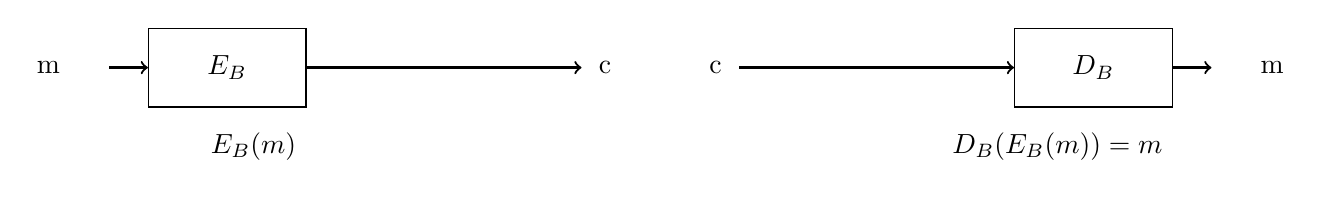
\begin{tikzpicture}
    % First set of text and boxes
    \node[anchor=east] at (0,0) {m};
    \node[draw, rectangle, minimum width=2cm, minimum height=1cm] (box1) at (2,0) {$E_B$};
    \node[anchor=east] at (3,-1) {$E_B(m)$};
    \node[anchor=west] at (8,0) {c};

    % Arrows
    \draw[->, thick] (0.5,0) -- (box1.west);
    \draw[->, thick] (box1.east) -- (6.5,0);

    % Second set of text and boxes
    \node[anchor=east] at (7,0) {c};
    \node[draw, rectangle, minimum width=2cm, minimum height=1cm] (box4) at (13,0) {$D_B$};
    \node[anchor=east] at (14,-1) {$D_B(E_B(m)) = m$};
    \node[anchor=west] at (15,0) {m};

    % Arrows
    \draw[->, thick] (8.5,0) -- (box4.west);
    \draw[->, thick] (box4.east) -- (14.5,0);

\end{tikzpicture}


  \centering   
\end{figure}

\subsection*{Method 2: Authenticity Ensured}
Lets say, person $A$ wants to send a message to person $B$. Now, person $A$ created the pair of keys $E_A$ and $D_A$ and sends $E_A$ publically.
So, now $A$ encrypts message $m$ using $D_A$ to send cipher $c$.\\S
Here, since $E_A$ is known by everyone including $B$, he can decrypt it using $E_A$. Thus here, authenticity is ensured as $D_A$ is private to person $A$ and only he/she can encrypt it. But, cipher $c$ can be decrypted by littrally everyone as $E_A$ is known publically. So security is not ensured.

\begin{figure}[ht]
  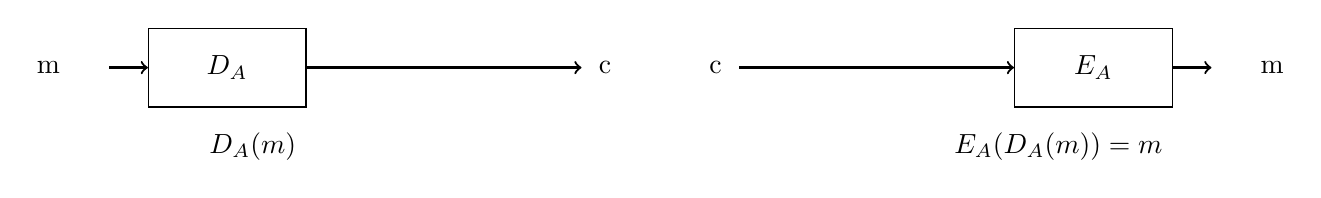
\begin{tikzpicture}
    % First set of text and boxes
    \node[anchor=east] at (0,0) {m};
    \node[draw, rectangle, minimum width=2cm, minimum height=1cm] (box1) at (2,0) {$D_A$};
    \node[anchor=east] at (3,-1) {$D_A(m)$};
    \node[anchor=west] at (8,0) {c};

    % Arrows
    \draw[->, thick] (0.5,0) -- (box1.west);
    \draw[->, thick] (box1.east) -- (6.5,0);

    % Second set of text and boxes
    \node[anchor=east] at (7,0) {c};
    \node[draw, rectangle, minimum width=2cm, minimum height=1cm] (box4) at (13,0) {$E_A$};
    \node[anchor=east] at (14,-1) {$E_A(D_A(m)) = m$};
    \node[anchor=west] at (15,0) {m};

    % Arrows
    \draw[->, thick] (8.5,0) -- (box4.west);
    \draw[->, thick] (box4.east) -- (14.5,0);

\end{tikzpicture}


  \centering   
\end{figure}

\subsection*{Method 3: Both Ensured}
What if we combine both the above methods to ensure both..\\
Lets say, person $A$ wants to send a message to person $B$.\\
Both of them creates pairs of keys $E_A$, $D_A$ and $E_B$, $D_B$ (and, $E_B$, $E_A$ are public).

\begin{figure}[ht]
  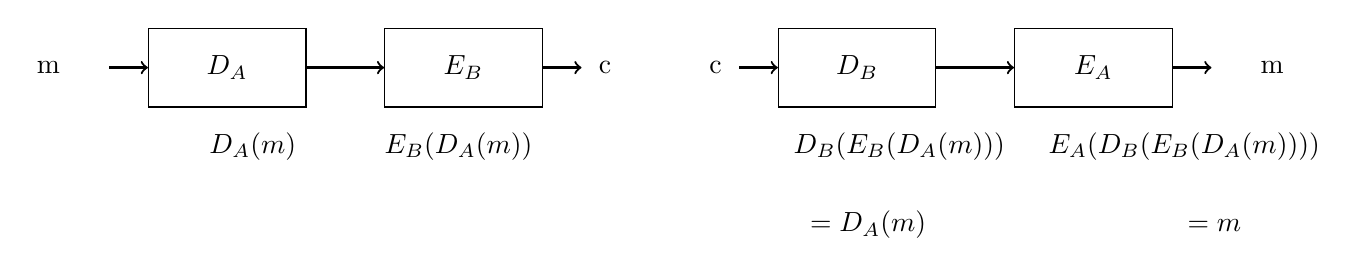
\begin{tikzpicture}
    % First set of text and boxes
    \node[anchor=east] at (0,0) {m};
    \node[draw, rectangle, minimum width=2cm, minimum height=1cm] (box1) at (2,0) {$D_A$};
    \node[anchor=east] at (3,-1) {$D_A(m)$};
    \node[draw, rectangle, minimum width=2cm, minimum height=1cm] (box2) at (5,0) {$E_B$};
    \node[anchor=east] at (6,-1) {$E_B(D_A(m))$};
    \node[anchor=west] at (8,0) {c};

    % Arrows
    \draw[->, thick] (0.5,0) -- (box1.west);
    \draw[->, thick] (box2.east) -- (6.5,0);

    % Second set of text and boxes
    \node[anchor=east] at (7,0) {c};
    \node[draw, rectangle, minimum width=2cm, minimum height=1cm] (box3) at (10,0) {$D_B$};
    \node[anchor=east] at (12,-1) {$D_B(E_B(D_A(m)))$};
    \node[anchor=east] at (11,-2) {$ = D_A(m)$};
    \node[draw, rectangle, minimum width=2cm, minimum height=1cm] (box4) at (13,0) {$E_A$};
    \node[anchor=east] at (16,-1) {$E_A(D_B(E_B(D_A(m))))$};
    \node[anchor=east] at (15,-2) {$ = m$};
    \node[anchor=west] at (15,0) {m};

    % Arrows
    \draw[->, thick] (8.5,0) -- (box3.west);
    \draw[->, thick] (box4.east) -- (14.5,0);
    \draw[->, thick] (box1.east) -- (box2.west);
    \draw[->, thick] (box3.east) -- (box4.west);

\end{tikzpicture}


  \centering   
\end{figure}
This suffices both authenticity and secracy. Here, its noteworthy that algorithm is known by everyone unlike the historical methods and just that the keys are kept secret.

\section*{Access Control}
Eg- MAC, DAC, RBAC, ABAC, etc are algorithms/methods used to enable access control. Lets understand this with an eg: \\
Lets say there is data stored in a database where only specific users can read and special users can edit it. Also, people should not be able to delete or scatter the information.
So, readers and modifiers should have their own specific keys.

\section*{Random Number Generation}
Its of two types:
\subsection*{True Random Number generator(TRNG)}
This is based on actual random events such as some hardware that changes drastically with outside conditions. It is truely random and can't be predicted.

\subsection*{Pseudo Random Number generator(PRNG)}
This is done algorithmic and could be predicted based on its previous values.

% 25 - 01 - 2024 LECTURE 5

\clearpage
\noindent\tbox{05}{
\begin{center}  
    \huge Lecture - 05 \\
    \Large Topic: Symmetric Crytopgraphy(Stream Cipher, LFSR)
\end{center}
}

\section*{Weekly Test 1 Solutions}
\subsection*{Question 2}
Given : \\
Length of code = 128 bits \\
Cost of a processor = Rs.1000 \\
Cap on cost of processors is Rs.10 crores. The performance of the processors is 10ns/code and follows Moore's law, i.e. it doubles in 24 months. The code is expected to be broken in 7 days. \\ \\
Solution: \\
In $n$ years, performance will increase by a factor of $2^{\frac{n}{2}}$. Therefore, 
\[
2^{128} codes \times \frac{10\times 10^{-9}s}{2^{\frac{n}{2}}} = \frac{10 crore}{1000} processors \times 7days \times 24hrs \times 60min \times 60s
\]
On solving, $n$ turns out to be approximately 130 years.

\section*{Symmetric Encryption: Stream Cipher}
The input is a stream of bits and the encryption takes place one bit at a time. It is easy to compute. \\ 
e.g.: One Time Pad which encrypts as follows
\begin{gather*}
    c_{i} = m_{i} \oplus k_{i} \\
    c_{i} = m_{i} + k_{i} \bmod 2
\end{gather*}

To use this encryption we need a random number generator to obtain k. True random numbers can be generated from physical phenomena. Rather, We are gonna generate pseudo-random numbers, i.e., random numbers generated algorithmically. One such method is LFSR.

\subsection*{Linear Feedback Shift Register}

LFSR is a shift register whose input bit is a \textbf{linear} function of two or more of the previous output bits.

\begin{figure}[ht]
\begin{center}
      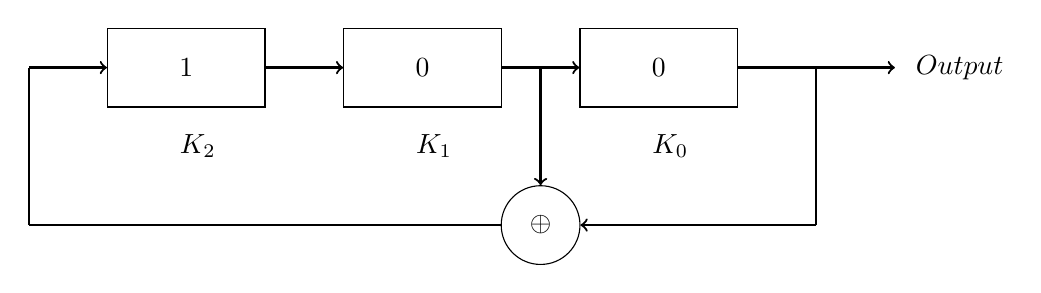
\begin{tikzpicture}
    % First set of text and boxes
    \node[draw, rectangle, minimum width=2cm, minimum height=1cm] (box1) at (2,0) {1};
    \node[anchor=east] at (2.5,-1) {$K_{2}$};
    \node[draw, rectangle, minimum width=2cm, minimum height=1cm] (box2) at (5,0) {0};
    \node[anchor=east] at (5.5,-1) {$K_{1}$};
    \node[draw, rectangle, minimum width=2cm, minimum height=1cm] (box3) at (8,0) {0};
    \node[draw, circle, minimum size=1cm] (xor1) at (6.5,-2) {$\oplus$};
    \node[anchor=east] at (8.5,-1) {$K_{0}$};
    \node[anchor=east] at (12.5,0) {$Output$};


    % Arrows
    \draw[->, thick] (0,0) -- (box1.west);
    \draw[->, thick] (box1.east) -- (box2.west);
    \draw[->, thick] (box2.east) -- (box3.west);
    \draw[->, thick] (box3.east) -- (11,0);
    \draw[-, thick] (10,0) -- (10,-2);
    \draw[->, thick] (10,-2) -- (xor1.east);
    \draw[->, thick] (6.5,0) -- (xor1.north);
    \draw[-, thick] (xor1.west) -- (0,-2);
    \draw[-, thick] (0,-2) -- (0,0);

\end{tikzpicture}
\end{center}

  \centering   
\end{figure}

The sequence generated by the given circuit is 
\begin{gather*}
    K_{i+3} = K_{i+1} \oplus K_{i} \\
    K_{i+3} = K_{i+1} + K_{i} \bmod 2\\
\end{gather*}
The expression for the input bit of an LFSR can be represented by a polynomial of degree $n$ ($n$ = number of registers), known as the characteristic polynomial. For example, the polynomial of the above LFSR circuit is
\begin{gather*}
x^{3} = x + 1 \bmod 2 \\
x^{3} + x + 1 \bmod 2 =0
\end{gather*}
Such a polynomial is called primitive if it is a factor of $x^{2^{n}-1}+1 \bmod 2$. A primitve polynomial generates a maximum length cycle of register values for given number of registers (cycle length = $2^{n}-1$, every pattern except 0). For example, the above polynomial generates the following series:\\
\[
100, 010, 101, 110, 111, 011, 001 
\]
of length $2^{3}-1 = 7$. Note that the polynomial is a factor of $x^{7}+1 \bmod 2$.
\[x^{2^{n}-1}+1 \bmod 2 = (x + 1)\times (x^{3} + x + 1)\times (x^{3} + x^{2} + 1)\bmod 2\]
To preserve randomness, the length of the cycle should be maximized, and so a primitive polynomial is preferred. Otherwise, we will end up generating a cyle of length less than $2^{n}-1$.\\

Here, the key depends on 
\begin{itemize}
    \item Characteristic polynomial
    \item \textbf{Seed} (Initial Value of the registers)
\end{itemize}

\subsection*{Programmable LFSR}
An LFSR circuit of degree $n$ that can configured to adopt any characteristic polynomial of the same degree. Here's an example of a programmable LFSR of degree 4.

\begin{center}
      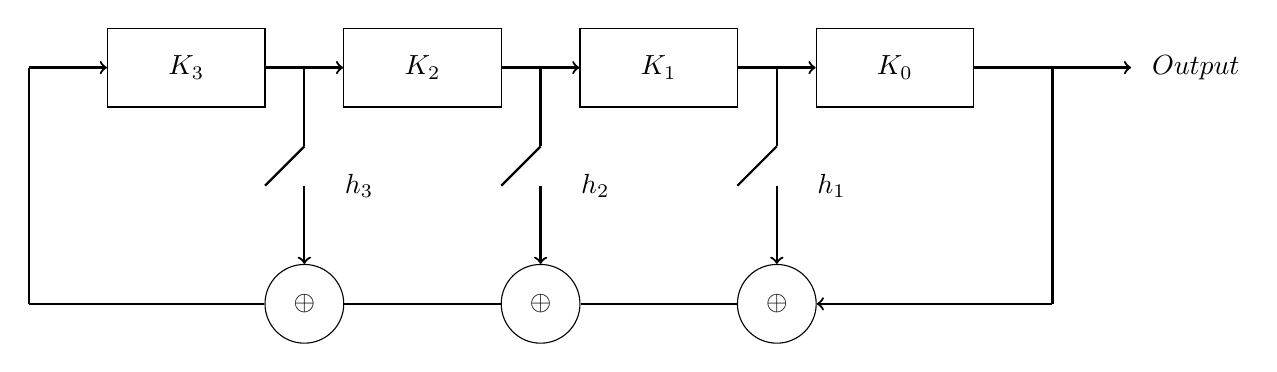
\begin{tikzpicture}
    % First set of text and boxes
    \node[draw, rectangle, minimum width=2cm, minimum height=1cm] (box1) at (2,0) {$K_{3}$};
    \node[anchor=east] at (4.5,-1.5) {$h_{3}$};
    \node[draw, rectangle, minimum width=2cm, minimum height=1cm] (box2) at (5,0) {$K_{2}$};
    \node[anchor=east] at (7.5,-1.5) {$h_{2}$};
    \node[draw, rectangle, minimum width=2cm, minimum height=1cm] (box3) at (8,0) {$K_{1}$};
    \node[anchor=east] at (10.5,-1.5) {$h_{1}$};
    \node[draw, rectangle, minimum width=2cm, minimum height=1cm] (box4) at (11,0) {$K_{0}$};
    \node[draw, circle, minimum size=1cm] (xor1) at (9.5,-3) {$\oplus$};
    \node[draw, circle, minimum size=1cm] (xor2) at (6.5,-3) {$\oplus$};
    \node[draw, circle, minimum size=1cm] (xor3) at (3.5,-3) {$\oplus$};
    \node[anchor=east] at (15.5,0) {$Output$};


    % Arrows
    \draw[->, thick] (0,0) -- (box1.west);
    \draw[->, thick] (box1.east) -- (box2.west);
    \draw[->, thick] (box2.east) -- (box3.west);
    \draw[->, thick] (box3.east) -- (box4.west);
    \draw[->, thick] (box4.east) -- (14,0);
    \draw[-, thick] (13,0) -- (13,-3);
    \draw[->, thick] (13,-3) -- (xor1.east);
    % tap1
    \draw[-, thick] (9.5,0) -- (9.5,-1);
    \draw[-, thick] (9.5,-1) -- (9,-1.5);
    \draw[->, thick] (9.5,-1.5) -- (xor1.north);
    % tap2
    \draw[-, thick] (6.5,0) -- (6.5,-1);
    \draw[-, thick] (6.5,-1) -- (6,-1.5);
    \draw[->, thick] (6.5,-1.5) -- (xor2.north);
    % tap3
    \draw[-, thick] (3.5,0) -- (3.5,-1);
    \draw[-, thick] (3.5,-1) -- (3,-1.5);
    \draw[->, thick] (3.5,-1.5) -- (xor3.north);
    \draw[-, thick] (xor1.west) -- (xor2.east);
    \draw[-, thick] (xor2.west) -- (xor3.east);
    \draw[-, thick] (xor3.west) -- (0,-3);
    \draw[-, thick] (0,-3) -- (0,0);

\end{tikzpicture}
\end{center}
The sequence generated by this would depend on the keys h1,h2,h3 as shown:
\begin{gather*}
        K_{i+4} = h_{3}K_{i+3} + h_{2}K_{i+2} + h_{1}K_{i+1} + K_{i} \bmod 2\\
\end{gather*}
Due to its linear nature, an LFSR can be easily broken.
We shall introduce non-linearity by using AND and OR gates in the circuit which will be covered in the next class :)

% 29 - 01 - 2024 LECTURE 6

\clearpage
\noindent\tbox{06}{
\begin{center}  
    \huge Lecture - 06 \\
    \Large Topic: DES, Feistel Cipher
\end{center}
}

\section*{Stream Cipher - Short Summary}

\begin{figure}[ht]
\begin{center}
\begin{tikzpicture}
      % First set of text and boxes
      \node[draw, circle, minimum size=1cm] (xor1) at (2,-2) {$\oplus$};
      \node[anchor=east] at (0,-2) {$m$};
      \node[anchor=north] at (2,0) {$k_{i}$};
      \node[anchor=west] at (4,-2) {$c_{i}$};
  
  
      % Arrows
      \draw[->, thick] (0,-2) -- (xor1.west);
      \draw[->, thick] (xor1.east) -- (4,-2);
      \draw[->, thick] (2,-0.5) -- (xor1.north);
  
\end{tikzpicture}
\end{center}

  \centering   
\end{figure}

\section*{Block Cipher}
Bundle of bits are fed. %\hfill DES

\begin{figure}[ht]
  \begin{center}
  \begin{tikzpicture}
        % First set of text and boxes
        \node[draw, rectangle, minimum width=2cm, minimum height=1cm] (box) at (2,-2) {};
        \node[anchor=east] at (0,-2) {$m$};
        \node[anchor=north] at (2,0) {$k$};
        \node[anchor=west] at (4,-2) {$c$};

        % DES
        \node[draw, rectangle, minimum width=2cm, minimum height=1cm] (box2) at (10,-2) {DES};
        \node[anchor=south] at (8,-2) {$m$};
        \node[anchor=north] at (8,-2) {64 $bit$};
        \node[anchor=south] at (10,0) {$k$};
        \node[anchor=north] at (10,0) {56 $bit$};
        \node[anchor=south] at (12,-2) {$c$};
        \node[anchor=north] at (12,-2) {64 $bit$};

        % Arrows
        \draw[->, thick] (0,-2) -- (box.west);
        \draw[->, thick] (box.east) -- (4,-2);
        \draw[->, thick] (2,-0.5) -- (box.north);
        % Arrows des
        \draw[->, thick] (8.5,-2) -- (box2.west);
        \draw[->, thick] (box2.east) -- (11.5,-2);
        \draw[->, thick] (10,-0.5) -- (box2.north);
    
  \end{tikzpicture}
  \end{center}
  
    \centering   
  \end{figure}

\subsection*{Principle}
\begin{figure}[ht]
  \begin{center}
  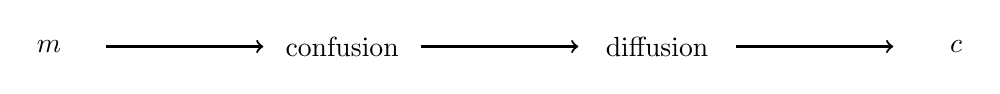
\begin{tikzpicture}
        % First set of text and boxes
        \node[anchor=west] at (0,0) {$m$};
        \node[anchor=center] at (4,0) {confusion};
        \node[anchor=center] at (8,0) {diffusion};
        \node[anchor=east] at (12,0) {$c$};
        % Arrows
        \draw[->, thick] (1,0) -- (3,0);
        \draw[->, thick] (5,0) -- (7,0);
        \draw[->, thick] (9,0) -- (11,0);
  \end{tikzpicture}
  \end{center}
  
    \centering   
  \end{figure}

% WRAPFIG
\begin{wrapfigure}{r}{0.5\textwidth}
  \begin{flushright}
    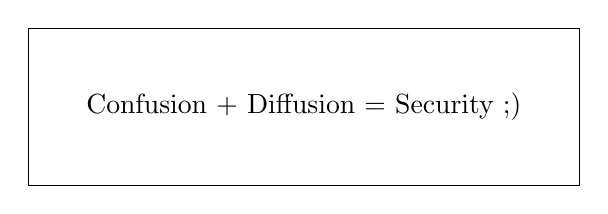
\begin{tikzpicture}
      \draw (0,0) rectangle (7,2);
      \node at (3.5,1) {Confusion + Diffusion = Security ;)};
    \end{tikzpicture}
    %\caption{Your TikZ figure caption here.}
  \end{flushright}
\end{wrapfigure}

The text undergoes several iterations of confusion and diffusion.

\subsubsection*{Confusion}
Relation between the text message and ciphertext is obscure.

\subsubsection*{Diffusion}
Change in one bit in the plaintext influences multiple bits in the ciphertext.

\vspace*{20pt}

\begin{figure}[h!]
  \begin{center}
  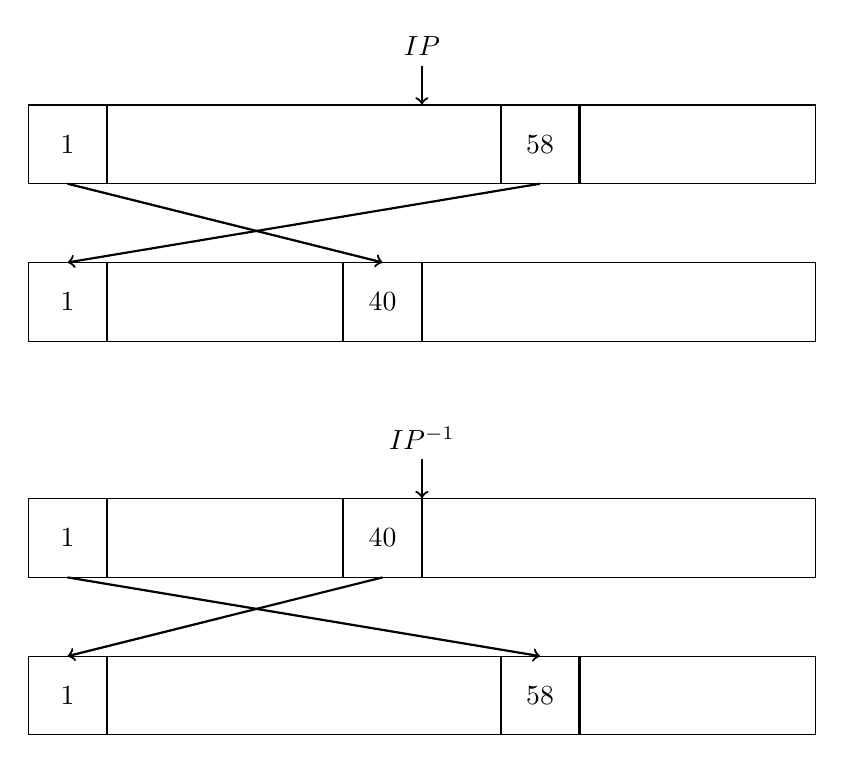
\begin{tikzpicture}
        % Boxes
        \node[anchor=south] at (5,-1) {$IP$};
        \node[draw, rectangle, minimum width=10cm, minimum height=1cm] (box1) at (5,-2) {};
        \node[draw, rectangle, minimum width=10cm, minimum height=1cm] (box2) at (5,-4) {};
        % lines and text in box1
        \node[anchor=center] at (0.5,-2) {1};
        \node[anchor=center] at (6.5,-2) {58};
        \draw[->, thick] (5,-1) -- (box1.north);
        \draw[-, thick] (1,-1.5) -- (1,-2.5);
        \draw[-, thick] (6,-1.5) -- (6,-2.5);
        \draw[-, thick] (7,-1.5) -- (7,-2.5);
        % lines bw the boxes
        \draw[->, thick] (0.5,-2.5) -- (4.5,-3.5);
        \draw[->, thick] (6.5,-2.5) -- (0.5,-3.5);
        % lines and text in box2
        \node[anchor=center] at (0.5,-4) {1};
        \node[anchor=center] at (4.5,-4) {40};
        \draw[-, thick] (1,-3.5) -- (1,-4.5);
        \draw[-, thick] (4,-3.5) -- (4,-4.5);
        \draw[-, thick] (5,-3.5) -- (5,-4.5);

        % Second set of boxes
        \node[anchor=south] at (5,-6) {$IP^{-1}$};
        \node[draw, rectangle, minimum width=10cm, minimum height=1cm] (box3) at (5,-7) {};
        \node[draw, rectangle, minimum width=10cm, minimum height=1cm] (box4) at (5,-9) {};
        % lines and text in box1
        \node[anchor=center] at (0.5,-7) {1};
        \node[anchor=center] at (4.5,-7) {40};
        \draw[->, thick] (5,-6) -- (box3.north);
        \draw[-, thick] (1,-6.5) -- (1,-7.5);
        \draw[-, thick] (4,-6.5) -- (4,-7.5);
        \draw[-, thick] (5,-6.5) -- (5,-7.5);
        % lines bw the boxes
        \draw[->, thick] (0.5,-7.5) -- (6.5,-8.5);
        \draw[->, thick] (4.5,-7.5) -- (0.5,-8.5);
        % lines and text in box2
        \node[anchor=center] at (0.5,-9) {1};
        \node[anchor=center] at (6.5,-9) {58};
        \draw[-, thick] (1,-8.5) -- (1,-9.5);
        \draw[-, thick] (6,-8.5) -- (6,-9.5);
        \draw[-, thick] (7,-8.5) -- (7,-9.5);

  \end{tikzpicture}
  \end{center}
  
    \centering   
  \end{figure}

\section*{Feistel Cipher}

% \begin{figure}[ht]
  \begin{figure}[ht]
  \begin{center}  
  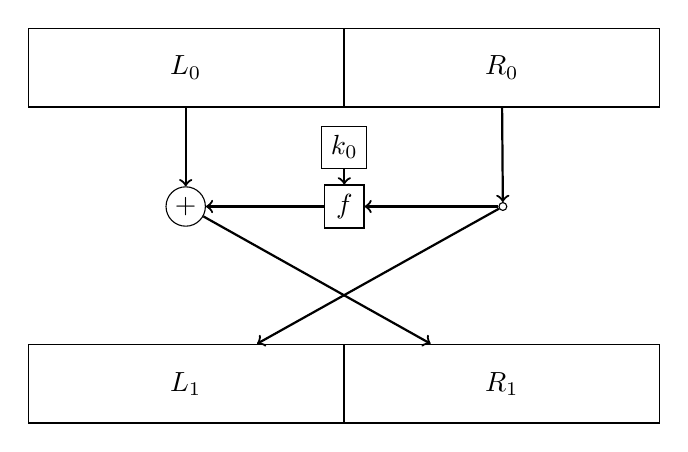
\begin{tikzpicture}[
    block1/.style={rectangle, draw, minimum width=4cm, minimum height=1cm, align=center},
    block2/.style={rectangle, draw, minimum width=0.5cm, minimum height=0.5cm, align=center},
    circlexor/.style={circle, draw, minimum size=0.5cm, inner sep=0pt},
    point/.style={circle, draw, minimum size=0.1cm, inner sep=0pt},
    arrow/.style={-Stealth, thick},
    node distance=2cm
  ]

    \node[block1] (L0) {$L_0$};
    \node[block1, right=0cm of L0] (R0) {$R_0$};
    \node[circlexor, below=1cm of L0] (xor) {+};
    \node[block1, below=3cm of L0] (L1) {$L_1$};
    \node[block1, right=0cm of L1] (R1) {$R_1$};
    \node[block2, right=1.5cm of xor] (f) {$f$};
    \node[block2, above=0.2cm of f] (k0) {$k_0$};
    \node[point, right=1.7cm of f] (point) {};

    \draw[->, thick] (L0) -- (xor);
    \draw[->, thick] (xor) -- (R1);
    \draw[->, thick] (R0) -- (point);
    \draw[->, thick] (point) -- (f);
    \draw[->, thick] (k0) -- (f);
    \draw[->, thick] (f) -- (xor);
    \draw[->, thick] (point) -- (L1);
  \end{tikzpicture}
  \end{center}
\end{figure}
% \end{figure}

% \begin{minipage}{0.45\textwidth}
  \begin{itemize}
    \item Left half(L0) is encrypted in one round and put on the right side(R1). 
    \item Right half(R0) is simply copied to the left side(L1). 
    \item The function f depends on the right half (here, R0) and the corresponding key of that round.
  \end{itemize}    
% \end{minipage}

\vspace*{100pt}
\subsection*{Function $f(K_{i+1},R_{i})$}

\begin{figure}[h!]
  \begin{center}
  \begin{tikzpicture}
        % Boxes
        \node[anchor=south] at (6,0) {$R_{i} (32 bit)$};
        \node[draw, rectangle, minimum width=2cm, minimum height=1cm] (box1) at (6,-1) {Expand};
        \draw[->, thick] (6,0) -- (box1.north);
        \node[draw, circle, minimum size=0.5cm] (xor1) at (6,-2.5) {$\oplus$};
        \node[anchor=west] at (7,-2.5) {$K_{i+1} (\text{48 bits from 56 bits key})$};\draw[->, thick] (7,-2.5) -- (xor1.east);
        \draw[->, thick] (box1.south) -- (xor1.north);\node[anchor=center] at (6.5,-3.5) {$48 bit$};
        % SUBSTITUTION PART
        \draw[-, thick] (xor1.south) -- (6,-4);
        \draw[-, thick] (0,-4) -- (12,-4);
        \draw[->, thick] (0,-4) -- (0,-5);\node[anchor=center] at (0.5,-4.5) {$6 bit$};
        \draw[->, thick] (1.5,-4) -- (1.5,-5);\node[anchor=center] at (2,-4.5) {$6 bit$};
        \draw[->, thick] (12,-4) -- (12,-5);\node[anchor=center] at (11.5,-4.5) {$6 bit$};
        %SUB BOXES
        \node[draw, rectangle, minimum width=1cm, minimum height=1cm] (s1) at (0,-6) {$S1$};
        \node[draw, rectangle, minimum width=1cm, minimum height=1cm] (s2) at (1.5,-6) {$S2$};
        \node[draw, rectangle, minimum width=1cm, minimum height=1cm] (s8) at (12,-6) {$S8$};
          %dots
          \fill[black] (3,-6) circle (1pt);
          \fill[black] (4.5,-6) circle (1pt);
          \fill[black] (6,-6) circle (1pt);
          \fill[black] (7.5,-6) circle (1pt);
          \fill[black] (9,-6) circle (1pt);
          \fill[black] (10.5,-6) circle (1pt);
        %lines again
        \node[draw, rectangle, minimum width=2cm, minimum height=1cm] (perm) at (6,-10) {$f(K_{i+1},R_{i})$};        
        \draw[->, thick] (6,-8) -- (perm.north);\node[anchor=center] at (6.5,-8.5) {$32 bits$};
        \draw[-, thick] (0,-8) -- (12,-8);
        \draw[-, thick] (0,-7) -- (0,-8);\node[anchor=center] at (0.5,-7.5) {$4 bit$};
        \draw[-, thick] (1.5,-7) -- (1.5,-8);\node[anchor=center] at (2,-7.5) {$4 bit$};
        \draw[-, thick] (12,-7) -- (12,-8);\node[anchor=center] at (11.5,-7.5) {$4 bit$};


  \end{tikzpicture}
  \end{center}
  
    \centering   
  \end{figure}

\subsection*{Expansion}
1 bit may expand to 1 or 2 bits.

\begin{figure}[ht]
  \begin{center}
  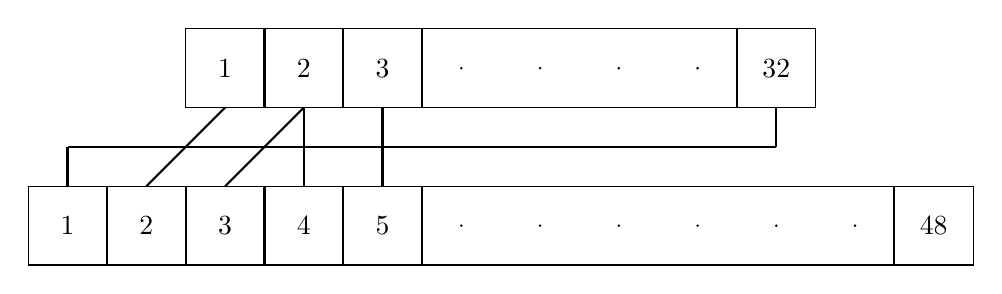
\begin{tikzpicture}
        % Boxes
        \node[draw, rectangle, minimum width=8cm, minimum height=1cm] (box1) at (6,0) {};
        \node[draw, rectangle, minimum width=12cm, minimum height=1cm] (box2) at (6,-2) {};
        % lines and text in box1
        \node[anchor=center] at (2.5,0) {1};
        \node[anchor=center] at (3.5,0) {2};
        \node[anchor=center] at (4.5,0) {3};
        \node[anchor=center] at (9.5,0) {32};
        \draw[-, thick] (3,0.5) -- (3,-0.5);
        \draw[-, thick] (4,0.5) -- (4,-0.5);
        \draw[-, thick] (5,0.5) -- (5,-0.5);
        \draw[-, thick] (9,0.5) -- (9,-0.5);
        % lines bw the boxes
        \draw[-, thick] (2.5,-0.5) -- (1.5,-1.5);
        \draw[-, thick] (3.5,-0.5) -- (2.5,-1.5);
        \draw[-, thick] (3.5,-0.5) -- (3.5,-1.5);
        \draw[-, thick] (4.5,-0.5) -- (4.5,-1.5);
        \draw[-, thick] (9.5,-0.5) -- (9.5,-1);
        \draw[-, thick] (0.5,-1) -- (9.5,-1);
        \draw[-, thick] (0.5,-1) -- (0.5,-1.5);

        % lines and text in box2
        \node[anchor=center] at (0.5,-2) {1};
        \node[anchor=center] at (1.5,-2) {2};
        \node[anchor=center] at (2.5,-2) {3};
        \node[anchor=center] at (3.5,-2) {4};
        \node[anchor=center] at (4.5,-2) {5};
        \node[anchor=center] at (11.5,-2) {48};
        \draw[-, thick] (1,-1.5) -- (1,-2.5);
        \draw[-, thick] (2,-1.5) -- (2,-2.5);
        \draw[-, thick] (3,-1.5) -- (3,-2.5);
        \draw[-, thick] (4,-1.5) -- (4,-2.5);
        \draw[-, thick] (5,-1.5) -- (5,-2.5);
        \draw[-, thick] (11,-1.5) -- (11,-2.5);
          %dots
          \fill[black] (5.5,0) circle (0.5pt);
          \fill[black] (6.5,0) circle (0.5pt);
          \fill[black] (7.5,0) circle (0.5pt);
          \fill[black] (8.5,0) circle (0.5pt);
          \fill[black] (6.5,-2) circle (0.5pt);
          \fill[black] (7.5,-2) circle (0.5pt);
          \fill[black] (8.5,-2) circle (0.5pt);
          \fill[black] (9.5,-2) circle (0.5pt);
          \fill[black] (10.5,-2) circle (0.5pt);
          \fill[black] (5.5,-2) circle (0.5pt);
        

  \end{tikzpicture}
  \end{center}
  
    \centering   
  \end{figure}

\subsection*{Substitution}
Substitution is done based on 8 tables(S1 to S8) of size 4$\times$16. The 6 bit input is used to navigate through the substitution table. The first and 
last bit indicates the row and the 4 bits in the middle indicate the column.

\subsection*{Key Generation}
The Key is of 56 bits, outta which every $7^{th}$ bit is redundant and thus discarded after shifting(to be precise, its rotation) as shown below.\\

\begin{figure}[ht]
  \begin{center}
  \captionsetup{labelformat=empty}
  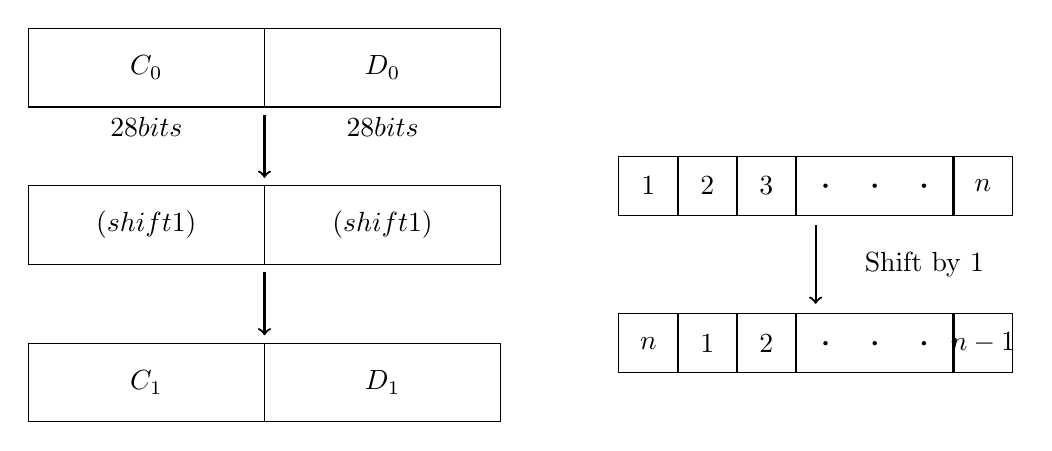
\begin{tikzpicture}
        % Boxes
        \node[draw, rectangle, minimum width=3cm, minimum height=1cm] (boxl1) at (1.5,0) {$C_{0}$};
        \node[draw, rectangle, minimum width=3cm, minimum height=1cm] (boxr1) at (4.5,0) {$D_{0}$};
        \node[draw, rectangle, minimum width=3cm, minimum height=1cm] (boxl2) at (1.5,-2) {$(shift1)$};
        \node[draw, rectangle, minimum width=3cm, minimum height=1cm] (boxr2) at (4.5,-2) {$(shift1)$};
        \node[draw, rectangle, minimum width=3cm, minimum height=1cm] (boxl1) at (1.5,-4) {$C_{1}$};
        \node[draw, rectangle, minimum width=3cm, minimum height=1cm] (boxr1) at (4.5,-4) {$D_{1}$};
        % lines and text in box1
        \node[anchor=south] at (1.5,-1) {$28 bits$};
        \node[anchor=south] at (4.5,-1) {$28 bits$};
        \draw[->, thick] (3,-0.6) -- (3,-1.4);
        \draw[->, thick] (3,-2.6) -- (3,-3.4);

        %LEFT SHIFT
        \node[draw, rectangle, minimum width=5cm, minimum height=0.75cm] (ls1) at (10,-1.5) {};
        \node[draw, rectangle, minimum width=5cm, minimum height=0.75cm] (ls2) at (10,-3.5) {};
        \draw[->, thick] (10,-2) -- (10,-3);
        \node[anchor=west] at (10.5,-2.5) {Shift by 1};
        %1
        \draw[-, thick] (8.25,-1.125) -- (8.25,-1.875);
        \draw[-, thick] (9,-1.125) -- (9,-1.875);
        \draw[-, thick] (9.75,-1.125) -- (9.75,-1.875);
        \draw[-, thick] (11.75,-1.125) -- (11.75,-1.875);
        \node[anchor=center] at (7.875,-1.5) {$1$};
        \node[anchor=center] at (8.625,-1.5) {$2$};
        \node[anchor=center] at (9.375,-1.5) {$3$};
        \node[anchor=center] at (12.125,-1.5) {$n$};

          %dots
          \fill[black] (10.125,-1.5) circle (0.8pt);
          \fill[black] (10.75,-1.5) circle (0.8pt);
          \fill[black] (11.375,-1.5) circle (0.8pt);
        
        %2
        \draw[-, thick] (8.25,-3.125) -- (8.25,-3.875);
        \draw[-, thick] (9,-3.125) -- (9,-3.875);
        \draw[-, thick] (9.75,-3.125) -- (9.75,-3.875);
        \draw[-, thick] (11.75,-3.125) -- (11.75,-3.875);
        \node[anchor=center] at (7.875,-3.5) {$n$};
        \node[anchor=center] at (8.625,-3.5) {$1$};
        \node[anchor=center] at (9.375,-3.5) {$2$};
        \node[anchor=center] at (12.125,-3.5) {$n-1$};

          %dots
          \fill[black] (10.125,-3.5) circle (0.8pt);
          \fill[black] (10.75,-3.5) circle (0.8pt);
          \fill[black] (11.375,-3.5) circle (0.8pt);
        

  \end{tikzpicture}
  \caption{Note : The left half and right half of first key are $C_{0}$ and $D_{0}$, respectively. Similarly, the second key comprises of $C_{1}$ and $D_{1}$.}
  \end{center}
  
    \centering   
  \end{figure}
Thus after rotating, we discard the 7th bits to get 48 bit keys for every corresponding round.
\begin{itemize}
  \item The keys for each round are generated by shifting from the preceding key.
  \item In rounds 1, 2, 9, and 16, shift occurs with an offset of 1, while for the remaining rounds, the offset is 2. 
\end{itemize}    



\clearpage
\noindent\tbox{07}{
\begin{center}  
    \huge Lecture - 07 \\
    \Large Topic: Decryption of DES and Assymetric Cryptography
\end{center}
}

Last class we saw about encryption in DES. Now lets see how to decrypt it.
\section*{Decryption in DES}
For decryption we just follow the exact same enryption method in reverse order. You may think that we need to calculate $f^{-1}$ which had expansion and contraction using s-boxes.
But actually, we don't need its inverse and we can use the same $f$ function.\\
\begin{align*}
  R_{i+1} &= L_i \oplus f(k_i,R_i) \\
  L_i \oplus R_{i+1} &= L_i \oplus L_i \oplus f(k_i,R_i) \\
  L_i \oplus R_{i+1} &= f(k_i,R_i) \text{ [$R_i = L_{i+1}$]}\\
  L_i \oplus R_{i+1} &= f(k_i,L_{i+1}) \text{ [$R_i = L_{i+1}$]}\\
  L_i &= R_{i+1} \oplus f(k_i,L_{i+1}) \\
\end{align*}
Thus, we get $L_i$ from $R_{i+1}$ and $L_{i+1}$.

\begin{figure}[ht]
  \begin{center}  
  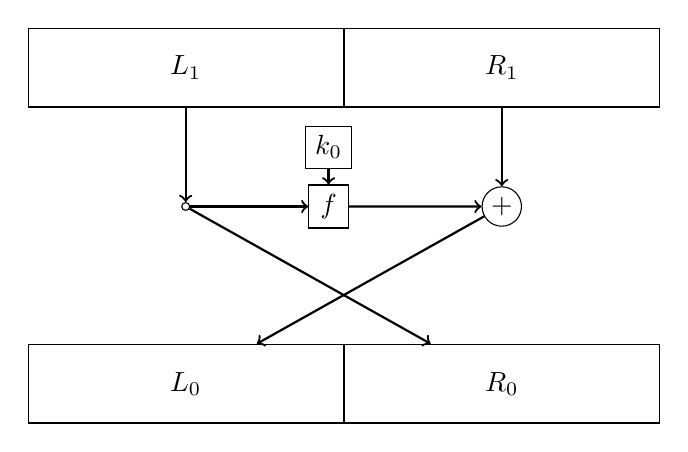
\begin{tikzpicture}[
    block1/.style={rectangle, draw, minimum width=4cm, minimum height=1cm, align=center},
    block2/.style={rectangle, draw, minimum width=0.5cm, minimum height=0.5cm, align=center},
    circlexor/.style={circle, draw, minimum size=0.5cm, inner sep=0pt},
    point/.style={circle, draw, minimum size=0.1cm, inner sep=0pt},
    arrow/.style={-Stealth, thick},
    node distance=2cm
  ]

    \node[block1] (L1) {$L_1$};
    \node[block1, right=0cm of L1] (R1) {$R_1$};
    \node[circlexor, below=1cm of R1] (xor) {+};
    \node[point, below=1.2cm of L1] (point) {};

    \node[block1, below=3cm of L1] (L0) {$L_0$};
    \node[block1, right=0cm of L0] (R0) {$R_0$};
    \node[block2, right=1.5cm of point] (f) {$f$};
    \node[block2, above=0.2cm of f] (k0) {$k_0$};

    \draw[->, thick] (R1) -- (xor);
    \draw[->, thick] (xor) -- (L0);
    \draw[->, thick] (L1) -- (point);
    \draw[->, thick] (point) -- (f);
    \draw[->, thick] (k0) -- (f);
    \draw[->, thick] (f) -- (xor);
    \draw[->, thick] (point) -- (R0);
  \end{tikzpicture}
  \end{center}
  \centering   
\end{figure}

As we have done the reverse, for 1 round, if we do it for 16 rounds, the final ouptut comes in $R_0$ and $L_0$ in reverse order and thus it should be reversed to get the original message.\\
Lets prove that its in reverse order. [d- denotes for bitstrings during decryption, and e- denotes encryption]
\begin{align*}
  L_0^d &= R_{16}^e \\
  R_0^d &= L_{16}^e = R_{15}^e \\
  L_1^d &= R_{0}^d = R_{15}^e \\
  R_1^d &= L_0^d \oplus f(R_0^d, k_1^d) \\
  &= L_0^d \oplus f(R_{15}^e, k_{16}^e) \\
  &= R_{16}^e \oplus f(R_{15}^e, k_{16}^e) \\
  &= L_{15}^e \oplus f(R_{15}^e, k_{16}^e) \oplus f(R_{15}^e, k_{16}^e) \\
  &= L_{15}^e \\
\end{align*}
thus, $R_1^d=L_{15}^e$ and similarly, $L_1^d=R_{15}^e$. so just the right and left are just reversed.

\section*{Problem with DES, and subsequent methods}
Here, since the key length is just 64 bits, brute force method was very much possible, and so other methods such as AES, DES were introduced.\\
\subsection*{AES(Advanced Encryption Standard)}
AES is a block cipher which encrypts 128 bits at a time. Its key length are 128 bits, 192, or 256 in different different methods. Correspondigly, 10 rounds, 12, and 14 rounds of encryption happens respectively.\\
Unlike  DES, here every operation is byte(8 bits) wise and not bit wise.\\
In every round, the following happens:
\begin{itemize}
  \item byte Substitution(by passing thorough s-blocks and stuffs)
  \item Row shift (for diffusion)
  \item Mix column (for diffusion)
  \item Key addition(xor with key)
\end{itemize}
Since they are byte wise operation, (i.e, {0,1,2,..,255}) finite field algebra would be useful to understand AES.
Galois field theory (GF(256)) - prof suggested to read this on our own.

\subsection*{3DES or TDES(triple DES)}
It can be done is two ways as shown:

\begin{figure}[ht]
  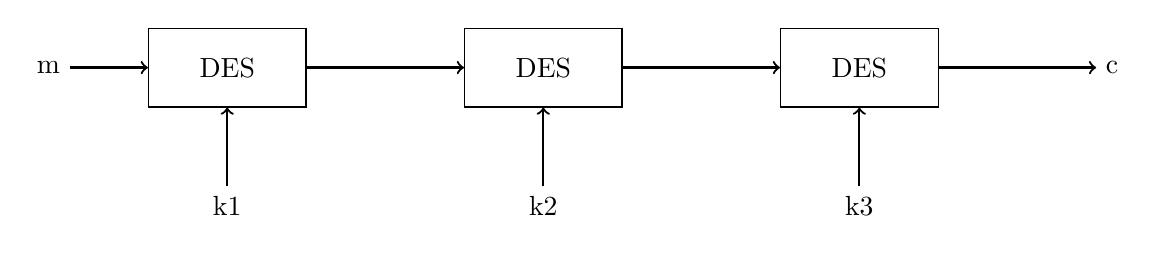
\begin{tikzpicture}
    % First set of text and boxes
    \node[anchor=east] (m) at (0,0) {m};
    \node[draw, rectangle, minimum width=2cm, minimum height=1cm] (des1) at (2,0) {DES};
    \node[draw, rectangle, minimum width=2cm, minimum height=1cm, right=2cm of des1] (des2) {DES};
    \node[draw, rectangle, minimum width=2cm, minimum height=1cm, right=2cm of des2] (des3) {DES};
    \node[right=2cm of des3] (c) {c};
    \node[below=1cm of des1] (k1) {k1};
    \node[below=1cm of des2] (k2) {k2};
    \node[below=1cm of des3] (k3) {k3};


    \draw[->, thick] (m) -- (des1.west);
    \draw[->, thick] (des1.east) -- (des2.west);
    \draw[->, thick] (des2.east) -- (des3.west);
    \draw[->, thick] (des3.east) -- (c);

    \draw[->, thick] (k1) -- (des1.south);
    \draw[->, thick] (k2) -- (des2.south);
    \draw[->, thick] (k3) -- (des3.south);

\end{tikzpicture}


  \centering   
\end{figure}

\begin{figure}[ht]
  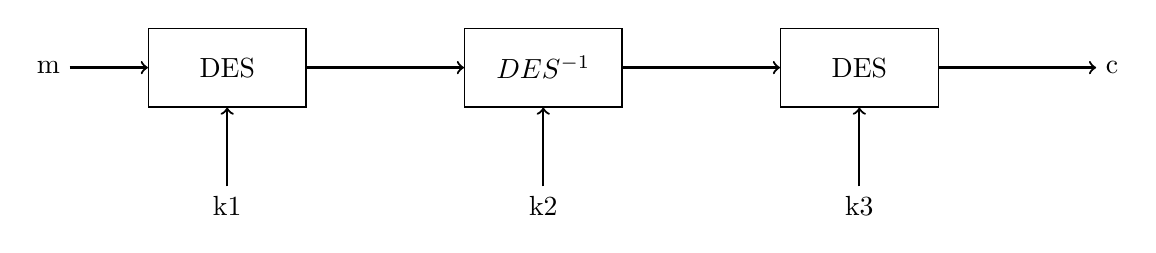
\begin{tikzpicture}
    % First set of text and boxes
    \node[anchor=east] (m) at (0,0) {m};
    \node[draw, rectangle, minimum width=2cm, minimum height=1cm] (des1) at (2,0) {DES};
    \node[draw, rectangle, minimum width=2cm, minimum height=1cm, right=2cm of des1] (des2) {$DES^{-1}$};
    \node[draw, rectangle, minimum width=2cm, minimum height=1cm, right=2cm of des2] (des3) {DES};
    \node[right=2cm of des3] (c) {c};
    \node[below=1cm of des1] (k1) {k1};
    \node[below=1cm of des2] (k2) {k2};
    \node[below=1cm of des3] (k3) {k3};


    \draw[->, thick] (m) -- (des1.west);
    \draw[->, thick] (des1.east) -- (des2.west);
    \draw[->, thick] (des2.east) -- (des3.west);
    \draw[->, thick] (des3.east) -- (c);

    \draw[->, thick] (k1) -- (des1.south);
    \draw[->, thick] (k2) -- (des2.south);
    \draw[->, thick] (k3) -- (des3.south);

\end{tikzpicture}


  \centering   
\end{figure}

\section*{Rivest–Shamir–Adleman (RSA) algorithm}
Its an Assymetric type encryption. The method is as follows.
\begin{itemize}
  \item get two large prime numbers p and q (let $p,q > 2^{1024}$)
  \item find $n = pq$
  \item euler's function $\phi(n) = (p-1)(q-1)$
  \item select public key $e$ such that, $gcd(e,\phi(n) = 1)$
  \item obtain private key $d$ which is $= e^{-1} \pmod{\phi(n)} $. Here, inverse element exist because $gcd(e,\phi(n)) = 1$.
\end{itemize}
private info - d,p,q \\
public info - e,N
\begin{itemize}
  \item[encrypt:] $c = m^e \pmod{n}$
  \item[decrypt:] 
  \begin{align*}
    c^d \pmod{n} &= (m^e)^d \pmod{n} \\
    &= m^{ed} \pmod{n} \\
    &= m^{q\phi(n) + 1} \pmod{n} \\
    &= m^{q\phi(n)}.m \pmod{n} \\
    &= m \text{      ;fermat's little theorem}
  \end{align*}
  fermat's little theorem - $a^{\phi(n)} \pmod{n} = 1$.
\end{itemize}
Generally, Assymetric key is computationally very expensive and thus very difficult to send the entire message through Assymetric method. Thus, keys of Symmetric key method are sent using Assymetric method and messages are sent with Symmetric key encryption henceforth.


\clearpage
\noindent\tbox{08}{
\begin{center}  
    \huge Lecture - 08 \\
    \Large Topic: RSA algorithm and Diffie–Hellman Key Exchange
\end{center}
}

\section*{Breaking RSA}
The main difficulty of breaking RSA algorithm lies in factorisation of $n$. As seen in previous lecture, if we could find $p$ and $q$ from $n$, then $\phi(n)$ can be found out. Using $e$ (Public key), $d$ can be found and thus could be decrypted by any Eavesdropper.
Thus factorisation is the only difficulty here.. In fact, such a factorisation is an open problem, if factorised, awards are awaiting.. See \href{https://en.wikipedia.org/wiki/RSA_Factoring_Challenge}{link}

\section*{Diffie–Hellman Key Exchange}
Decide on prime number $p$ and a primive root $\alpha$(Primive root will be explained later. For now, assume its a number from 1 to $p-1$). Both these are public info.
\begin{figure}[ht]
  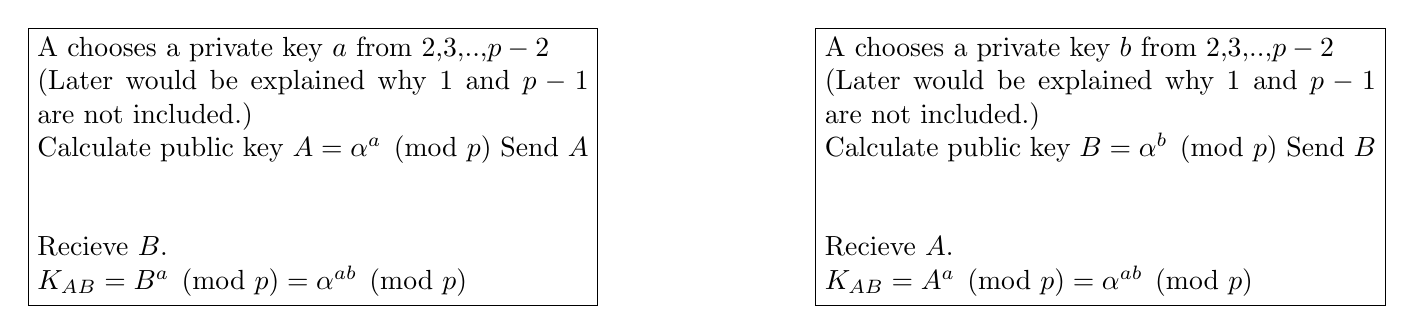
\begin{tikzpicture}
    % First set of text and boxes
    \node[draw, rectangle, minimum width=5cm, minimum height=1cm,anchor=east] (A) at (0,0) {
      \begin{minipage}{7cm}
        A chooses a private key $a$ from {2,3,..,$p-2$}\\ (Later would be explained why 1 and $p-1$ are not included.) \\
        Calculate public key $A = \alpha^a \pmod{p}$
        Send $A$ \\ \\ \\
        Recieve $B$.\\
        $K_{AB} = B^{a} \pmod{p} = \alpha^{ab} \pmod{p}$
      \end{minipage}
    };
    \node[draw, rectangle, minimum width=5cm, minimum height=1cm,anchor=east] (B) at (10,0) {
      \begin{minipage}{7cm}
        A chooses a private key $b$ from {2,3,..,$p-2$}\\ (Later would be explained why 1 and $p-1$ are not included.) \\
        Calculate public key $B = \alpha^b \pmod{p}$
        Send $B$ \\ \\ \\
        Recieve $A$.\\
        $K_{AB} = A^{a} \pmod{p} = \alpha^{ab} \pmod{p}$
      \end{minipage}
    };

    % \draw[->, thick] (7,-4) -- (10, -7);
    % \draw[->, thick] (10, -4) -- (7,-7);

\end{tikzpicture}

\centering   
\end{figure}

Now, using $K_{AB}$, Symmetric Cryptography techniques can be applied to send long messages.

\section*{Breaking DHP(Diffie–Hellman Problem)}
Eavesdropper knows $\alpha, p, A, B$. The only unknown things are $a,b$.\\
\begin{align*}
  A &= \alpha^{a} \pmod{p} \\
  a &= log_{\alpha}^{A} \pmod{p} \\
\end{align*}
Solving this Discrete Logarithm Problem(DLP) is computationally very hard.

\subsection*{Group Theory}
A group is a set of elements and an operator * such that it follows the following properties:
\begin{itemize}
  \item Closure property: if $a,b \in G, a * b = c \in G$
  \item Associativity
  \item existance of neutral element(identity element)
  \item existance of inverse element
\end{itemize}
(Commutativity is not necessary but if there, its called an abelian group)

\section*{How to choose $\alpha$}
Here, lets define a group $\mathbb{Z}^{*}_{p} = \{i: i \in {0,1,..,p-1}, gcd(i,p) = 1\}$ with operator as multiplication in $\pmod{p}$.\\
If p is a prime number, then $\mathbb{Z}^{*}_{p} = \{i: i \in {1,..,p-1}, gcd(i,p) = 1\}$ \\
Euler's function, $\phi(p) = |\mathbb{Z}^{*}_{p}| = p-1$ for a prime number. \\
Fermat's little theorem states that, $a^{\phi(n)} \pmod{n} = 1$ for any n. So here,
$\alpha^{\phi(p)} \pmod{p} = \alpha^{p-1} \pmod{p} = 1$ \\
i.e, on powering $\alpha$ repeats in a cycle of length, a factor of $\phi(p) = p-1$.
If the length is exactly $p-1$, we say its a primitive root of p.
We want the length to be as long as possible to maximise randomness, and number of possiblities of $\alpha^n$.\\
Eg - in $\mathbb{Z}^{*}_{11}$, 2 is a primitive root whereas, 3 is not.. 3 has a cycle of 5, and 2 has a cycle of 10 (= 11-1). Try it out.
\\ \\ \\
Why are $a$ and $b$ chosen from \{2,3,..,$p-2$\}, i.e, 1 and $p-1$ are ignored?\\
\textbf{If a = 1}, $A = \alpha^1 \pmod{p} = \alpha$. Since $A$ and $\alpha$ are known, its easily seen that they're equal and so $a=1$ can be found. Then, $K_{AB} = B^a = B$ simply. Thus key get knowned.\\
\textbf{If a = p-1}, $A = \alpha^{p-1} \pmod{p} = 1$(Fermat's little theorem). Since $A=1$, its easily seen that they're equal and so $a=p-1$ can be found, provided $\alpha$ is a primitve root. Otherwise, $a$ will be a factor of $p-1$ which also could be found easily ig.. Then, $K_{AB} = B^a$ simply. Thus key get knowned.\\



\clearpage% Lecture 9 on 09 - 02 - 2024
\noindent\tbox{09}{
\begin{center}  
    \huge Lecture - 09 \\
    \Large Topic: Diffie-Hellman Key Exchange Protocol (DHD), Elgamal
\end{center}
}

\section*{Diffie-Hellman Key Exchange}
Say there are two parties A and B that want to communicate: \\
Public info : p, $\alpha$ \\
\begin{multicols}{2}
Party A \\
$K_{private(A)} = a \in {2,3,...,p-2}$ \\ 
$K_{public(A)} = A = \alpha^{a}\pmod{p}$ \\ 
\columnbreak \\
Party B \\
$K_{private(B)} = b \in {2,3,...,p-2}$ \\ 
$K_{public(B)} = B = \alpha^{b}\pmod{p}$ \\ 
\end{multicols}

\begin{alignat*}{2}
&\xrightarrow[\hspace{1cm}]{\text{A}} K_{AB} = A^{b} \pmod{p} \\
&\quad\quad\quad =\alpha^{ab}\pmod{p} \\ 
K_{AB} = B^{a} \pmod{p} &\xleftarrow[\hspace{1cm}]{\text{B}} \\
=\alpha^{ab}\pmod{p} \\ 
c = m.K_{AB}\pmod{p} &\xrightarrow[\hspace{1cm}]{\text{c}} m = c.K_{AB}\pmod{p} \\
\end{alignat*}

\section*{Elgamal(1985)}



\clearpage% Lecture 10 on 12 - 02 - 2024
\noindent\tbox{10}{
\begin{center}  
    \huge Lecture - 10 \\
    \Large Topic: Digital Signatures - RSA
\end{center}
}

\section*{Security Objective(CIA)}
\begin{itemize}
  \item Confidentiality is reqd. Encryption using a key ensures confidentiality in fact as they can be decrypted only people with the key.
  \item \textbf{Integrity:} Message shold not be tampered in between. We should be able to identify if its tampered or not.
  \item \textbf{Message Authentication:} It should be provable that only the intended sender sent the message and no one else.
  \item \textbf{Non-repudiation:} If someone sent a message, later it can be proved that none other than him/her sent it. Eg- signature. Like if signed, later they cannot deny that they didn't send it.
  \item \textbf{Access Control:} Who all can read the message, who all can modify it, etc should be able to be controled.
\end{itemize}

\section*{Digital Signatures}
Similar to normal Signatures but are done on digital documents. It provides the above parameters including authentication and non-repudiation.
\subsection*{How to create digital signatures?}
Say a document carrying message $m$ is there and signature $s$. Message and signature are from "Message space" and "Signature space" resp (basically superset of messages and signatures).
Person $A$ is the owner and $B$ checks the signature. \\
$B$ calculates the sign of the document using key $k$ i.e, $Sig(m)$ and checks if its same as $S$ or not. If its same, then signature is verified and otherwise no.\\
If its document is tampered, calculated signature won't be same and could be identified that its tampered.\\
But this does not ensure Non-repudiation as anyone can find $Sig(m)$.\\ \\
To include Non-repudiation, Assymetric Key distribution can be used, where private key is used to find $S$ and it can only be verified by public key and signature cannot be calculated by it.

\section*{Digital Signature using RSA}
\textbf{Private info(i.e owner):} $d$, $p$, $q$, $n = pq$, signature $S = m^d \pmod{n}$. Now, $e = d^{-1} \pmod{\phi(n)}$, $n$, and $S$ are sent \\ \\
\textbf{Public info(i.e verifier):} $m$ ,$n$ , $S$, $e$. \\ $S^{e} \pmod{n}$ is calculated and if its equal to $m$, then its verified and not verified otherwise. \\

\textbf{What does attacker wants to do?:} \\
Message is known to everyone(like everyone knows A send 1000 rs to C), but what an attacker wants to do is that, he wants to change the message to $m'$ (say change 1000 to 10000 rs). Now, to calculate signature $S'$, $d$ is required. Say he made up some random $d$.
Since, $\phi(n)$ is unknown, $e$ cannot be calculated, and thus $e$ can't be send.

\section*{Digital Signatures using Elgamal}

\begin{figure}[ht]
  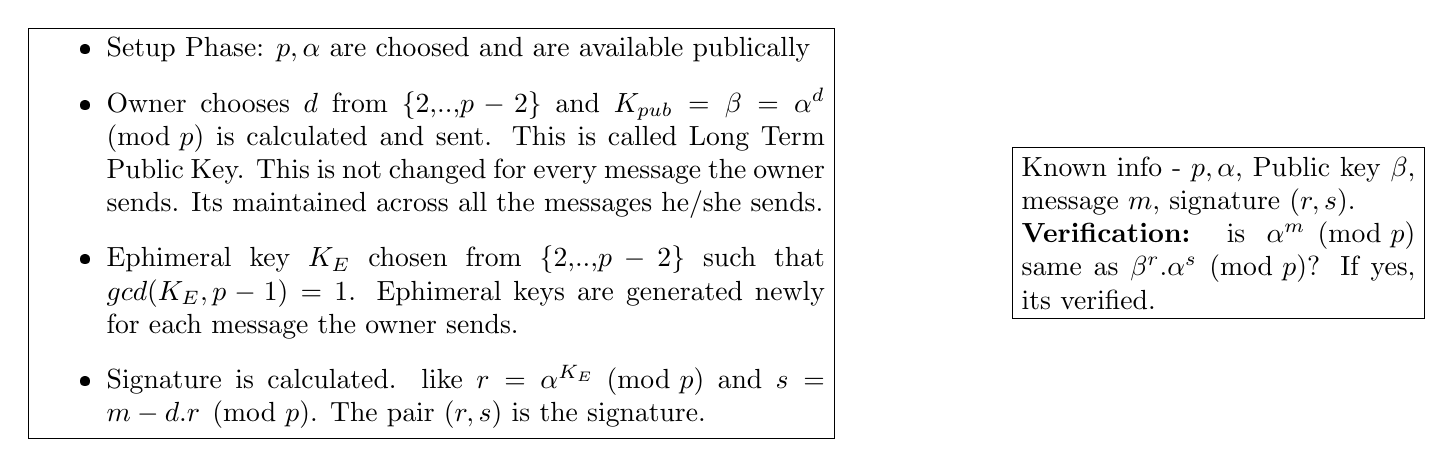
\begin{tikzpicture}
    % First set of text and boxes
    \node[draw, rectangle, minimum width=10cm, minimum height=1cm] (A) at (0,0) {
      \begin{minipage}{10cm}
        \begin{itemize}
          \item Setup Phase: $p,\alpha$ are choosed and are available publically
          \item Owner chooses $d$ from \{2,..,$p-2$\} and $K_{pub} = \beta = \alpha^d \pmod{p}$ is calculated and sent. This is called Long Term Public Key. This is not changed for every message the owner sends. Its maintained across all the messages he/she sends.
          \item Ephimeral key $K_E$ chosen from \{2,..,$p-2$\} such that $gcd(K_E,p-1) = 1$. Ephimeral keys are generated newly for each message the owner sends.
          \item Signature is calculated. like $r = \alpha^{K_E} \pmod{p}$ and $s = m-d.r \pmod{p}$. The pair $(r,s)$ is the signature.
        \end{itemize}
      \end{minipage}
    };
    \node[draw, rectangle, minimum width=5cm, minimum height=1cm] (B) at (10,0) {
      \begin{minipage}{5cm}
        Known info - $p, \alpha$, Public key $\beta$, message $m$, signature $(r,s)$.\\
        \textbf{Verification:} is $\alpha^m \pmod{p}$ same as $\beta^r.\alpha^s \pmod{p}$? If yes, its verified.
      \end{minipage}
    };

    % \draw[->, thick] (7,-4) -- (10, -7);
    % \draw[->, thick] (10, -4) -- (7,-7);

\end{tikzpicture}

\centering   
\end{figure}

\subsection*{Correctness}
\begin{align*}
  \beta^r.\alpha^s \pmod{p} &= \beta^r.\alpha^{m-d.r} \pmod{p} \\
  &= \alpha^{d.r}.\alpha^{m-d.r} \pmod{p} \\
  &= \alpha^{m} \pmod{p}
\end{align*}
Now, if someone wants to tamper the message, say they wants to create signature of the owner of different message $m'$.\\
$r = \alpha^{K_E}$ can be calculated by choosing some random $K_E$. But to calculate $s$, $d$ is required which can't be solved from the eqation $\beta = \alpha^d \pmod{p}$ due to discrete logarithmic problem.

\subsection*{Disadvantage}
The signature size is double the size of RSA as we are sending both $r$ and $s$ as signatures.



\clearpage% Lecture 10 on 15 - 02 - 2024
\noindent\tbox{11}{
\begin{center}  
    \huge Lecture - 11 \\
    \Large Topic: Digital Signatures Algorithm
\end{center}
}

\section*{Digital Signature Algorithm}
This is currently widely used methof for Digit Signatures. This algorithm reduces the size of the signature from 2048 to 320 bits and 4096 to 422 bits as compared to Elgamal method.\\

\begin{figure}[ht]
  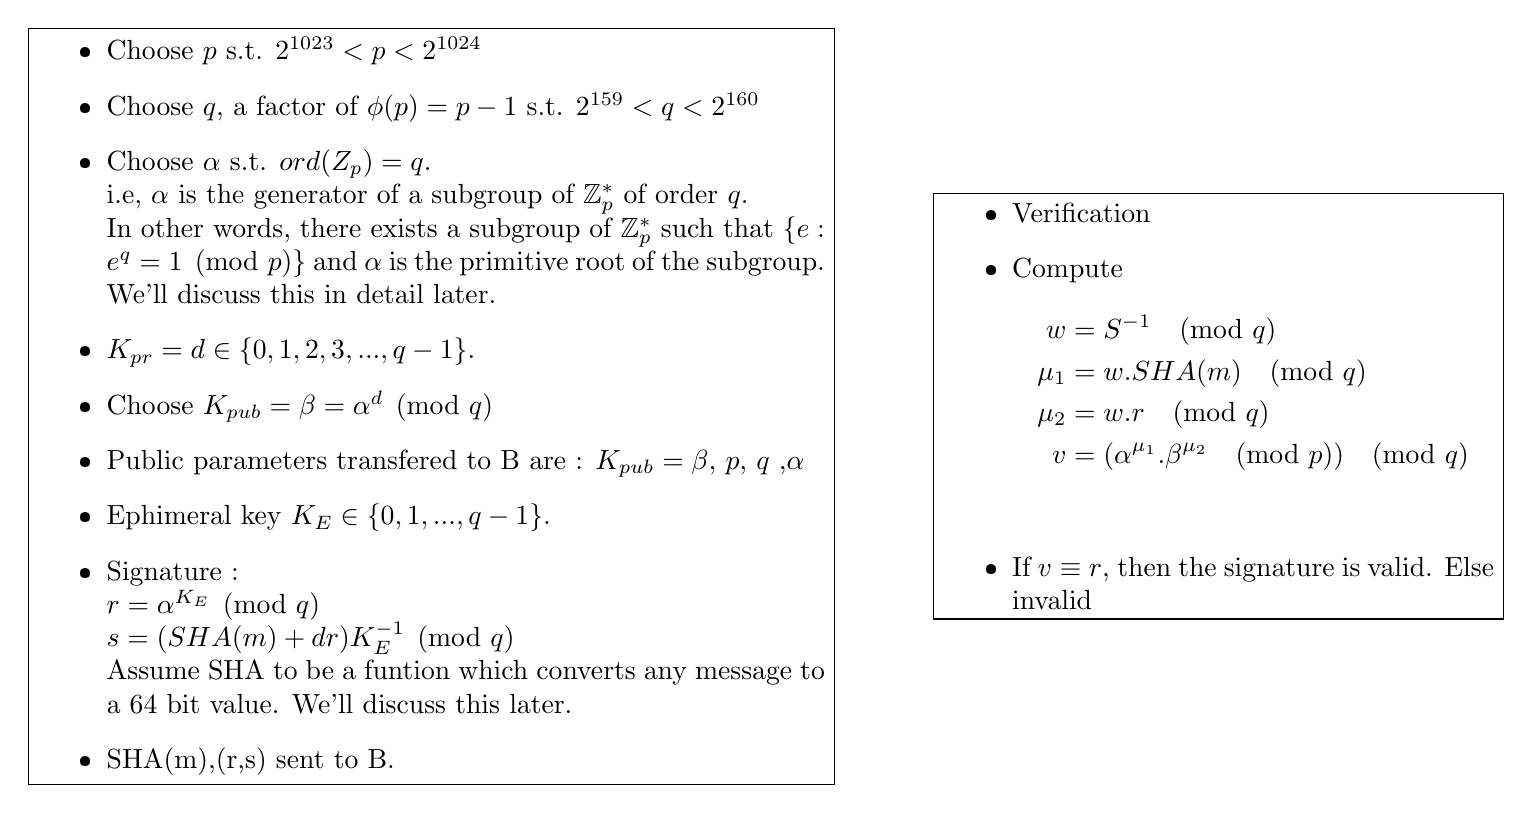
\begin{tikzpicture}
    % First set of text and boxes
    \node[draw, rectangle, minimum width=10cm, minimum height=1cm] (A) at (0,0) {
      \begin{minipage}{10cm}
        \begin{itemize}
          \item Choose $p$ s.t. $2^{1023}<p<2^{1024}$
          \item Choose $q$, a factor of $\phi(p) = p-1$ s.t. $2^{159}<q<2^{160}$
          \item Choose $\alpha$ s.t. $ord(Z_{p}) = q$. \\ i.e, $\alpha$ is the generator of a subgroup of $\mathbb{Z}^*_p$ of order $q$. \\ In other words, there exists a subgroup of $\mathbb{Z}^*_p$ such that $\{ e : e^q = 1 \pmod{p} \} $ and $\alpha$ is the primitive root of the subgroup. We'll discuss this in detail later.
          \item $K_{pr} = d \in \{0,1,2,3,...,q-1\}$.
          \item Choose $K_{pub} = \beta = \alpha^{d} \pmod{q}$
          \item Public parameters transfered to B are : $K_{pub} = \beta$, $p$, $q$ ,$\alpha$
          \item Ephimeral key $K_{E} \in \{0,1,...,q-1\}$.
          \item Signature : \\
          $r = \alpha^{K_{E}} \pmod{q}$ \\
          $s = (SHA(m)+dr) K_{E}^{-1} \pmod{q}$ \\ Assume SHA to be a funtion which converts any message to a 64 bit value. We'll discuss this later.
          \item SHA(m),(r,s) sent to B.
        \end{itemize}
      \end{minipage}
    };
    \node[draw, rectangle, minimum width=5cm, minimum height=1cm] (B) at (10,0) {
      \begin{minipage}{7cm}
        \begin{itemize}
          \item Verification
          \item Compute
          \begin{align*}
            w &= S^{-1} \pmod{q} \\
            \mu_{1} &= w.SHA(m) \pmod{q} \\
            \mu_{2} &= w.r \pmod{q} \\
            v &= (\alpha^{\mu_{1}}.\beta^{\mu_{2}} \pmod{p}) \pmod{q} \\
            \end{align*}
          \item If $v \equiv r$, then the signature is valid. Else invalid
        \end{itemize}
      \end{minipage}
    };

    % \draw[->, thick] (7,-4) -- (10, -7);
    % \draw[->, thick] (10, -4) -- (7,-7);

\end{tikzpicture}

\centering   
\end{figure}
$r,s$ are 160 bits each, and thus, the signature $(r,s)$ is of 320 bits (much smaller as compared to Elgamal method of $1024 + 1024 = 2048$ bits.)
\subsection*{Correctness}

\begin{align*}
  s &= (SHA(m)+d.r) K_{E}^{-1} \pmod{q} \\
  s.s^{-1}&= (SHA(m)+d.r) K_{E}^{-1} s^{-1} \pmod{q} \\
  1 &= (SHA(m)+d.r) K_{E}^{-1} s^{-1} \pmod{q} \\
  s^{-1}.(SHA(m)+d.r) &= K_E \pmod{q} \\
\end{align*}
So, $s^{-1}.(SHA(m)+d.r) = \theta q + K_E$.
\begin{align*}
  v &= \alpha^{s^{-1}SHA(m)} \beta^{s^{-1}r} \pmod{p} \pmod{q}\\
  &= \alpha^{s^{-1}SHA(m)} \alpha^{s^{-1}r.d} \pmod{p} \pmod{q}\\
  &= \alpha^{s^{-1}SHA(m)+s^{-1}r.d} \pmod{p} \pmod{q}\\
  &= \alpha^{s^{-1}(SHA(m)+r.d)} \pmod{p} \pmod{q}\\
  &= \alpha^{\theta q + K_E} \pmod{p} \pmod{q}\\
  &= (\alpha^{q})^{\theta}.\alpha^{K_E} \pmod{p} \pmod{q}\\
  &= \alpha^{K_E} \pmod{p} \pmod{q} \text{     [as $\alpha^q = 1 \pmod{p}$]}\\
  &= \alpha^{K_E} \pmod{q} \\
  &= r
\end{align*}
Here too, as $d$ is unknown signature can't be created by a random person other than the owner.

\subsection*{Clearing some concepts}
Subgroup of $\mathbb{Z}^*_p$ such that $\{ e : e^q = 1 \pmod{p} \} $ and $\alpha$ is the generator of the subgroup. Here, first notice that its a group on its own as the properties such as Closure, Associativity, etc exists.\\
Does inverse element exist?\\
We know that $e^{-1}$ exits in $\mathbb{Z}^*_p$. We just need to prove $e^{-1}$ is in the subset provided $e$ is in it.
\begin{align*}
  (e^{-1})^q &= x \pmod{p} \\
  e^q . (e^{-1})^q &= e^q . x \pmod{p} \\
  (e . e^{-1})^q &= 1 . x \pmod{p} \\
  1 &= x \pmod{p} \\
  x &= 1\\
\end{align*}
Thus proved $e^{-1}$ is in the subset. Thus proved that this subset is actually a group. \\
So just choose a primitive root $\alpha$ from this subgroup. \\ \\
SHA is a hashing funtion which creates any message to a 64 bit value. It hashes so widely such that, practically every message hashes to a different value. Though through pigeion hole principle, there will exist messages to hashing to same value mathematically, practically we can assume they hash to different values.\\ \\
Why do we hash the funtion? why can't we use the message at itself?\\
First, hashing increases confusion in message, i.e, even if just a small change is made in message, its hash would be completely different. Secondly, messages can be arbitarily long, and so to have it standard, we hash it to 64 bit value.



\clearpage% Lecture 10 on 15 - 02 - 2024
\noindent\tbox{12}{
\begin{center}  
    \huge Lecture - 12 \\
    \Large Topic: Digital Signatures Algorithm
\end{center}
}

\section*{Key Exchange}
Two parties $A$ and $B$ wants to exchange key between them to use Symmetric Cryptography from then as Assymetric algorithm is computationally expensive to send the whole message.\\
\textbf{Passive Eavesdropping:} Just can listen on the common commutication channel between two parties and cannot send data.\\
\subsection*{Active Eavesdropping}
Say an intruder is Active eavesdropper, i.e, he/she can listen to the common communication channel and also write or transfer messages.\\
Such an attack is called \textit{Man In The Middle} attack. Take example of DHKE between people $A$ and $B$. So, when $A=\alpha^{a}\pmod{p}$ and $B$ are transfered from each other, the intruder reads them, modify them as $A'$ and $B'$ and send to each other.\\
\begin{figure}[ht]
  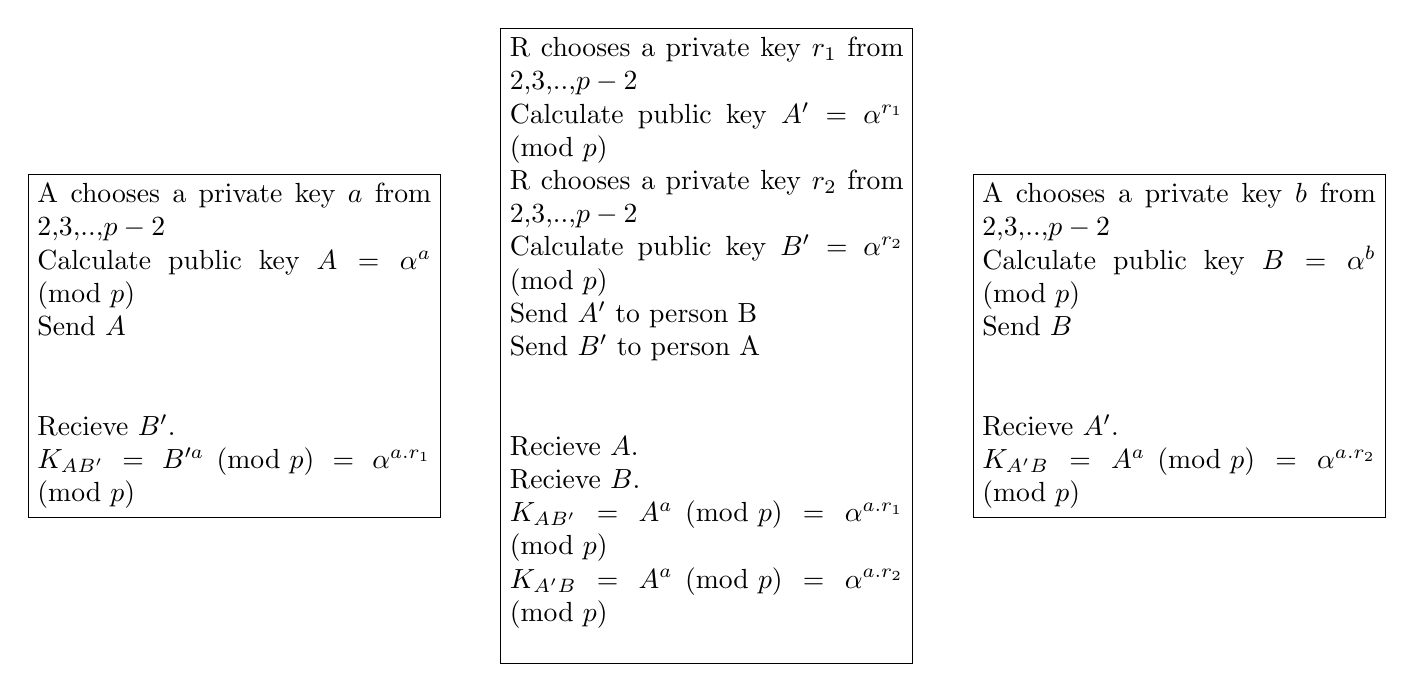
\begin{tikzpicture}
    % First set of text and boxes
    \node[draw, rectangle, minimum width=5cm, minimum height=1cm,anchor=east] (A) at (0,0) {
      \begin{minipage}{5cm}
        A chooses a private key $a$ from {2,3,..,$p-2$} \\
        Calculate public key $A = \alpha^a \pmod{p}$ \\
        Send $A$ \\ \\ \\
        Recieve $B'$.\\
        $K_{AB'} = B'^{a} \pmod{p} = \alpha^{a.r_1} \pmod{p}$
      \end{minipage}
    };
    \node[draw, rectangle, minimum width=5cm, minimum height=1cm,anchor=east] (R) at (6,0) {
      \begin{minipage}{5cm}
        R chooses a private key $r_1$ from {2,3,..,$p-2$} \\
        Calculate public key $A' = \alpha^{r_1} \pmod{p}$\\
        R chooses a private key $r_2$ from {2,3,..,$p-2$} \\
        Calculate public key $B' = \alpha^{r_2} \pmod{p}$ \\
        Send $A'$ to person B \\
        Send $B'$ to person A \\ \\ \\
        Recieve $A$.\\
        Recieve $B$.\\
        $K_{AB'} = A^{a} \pmod{p} = \alpha^{a.r_1} \pmod{p}$ \\
        $K_{A'B} = A^{a} \pmod{p} = \alpha^{a.r_2} \pmod{p}$ \\
      \end{minipage}
    };
    \node[draw, rectangle, minimum width=5cm, minimum height=1cm,anchor=east] (B) at (12,0) {
      \begin{minipage}{5cm}
        A chooses a private key $b$ from {2,3,..,$p-2$} \\
        Calculate public key $B = \alpha^b \pmod{p}$ \\
        Send $B$ \\ \\ \\
        Recieve $A'$.\\
        $K_{A'B} = A^{a} \pmod{p} = \alpha^{a.r_2} \pmod{p}$
      \end{minipage}
    };

    % \draw[->, thick] (7,-4) -- (10, -7);
    % \draw[->, thick] (10, -4) -- (7,-7);

\end{tikzpicture}

\centering   
\end{figure}
\\
Both the parties can't even identify that such an intruder is present in between. Person A assumes $B'$ was sent by actual person B and vice versa. Once, such a thing is done, the intruder can not only read the messages sent between them, but also can modify and send messages between them.\\
Very similar attack is possible even in Elgamal. This problem arrises because, there is no authentication for any message. To resolve authentication, one may think we can use digital signatures. But, that is also prone to such a middle man attack.

\section*{Centralized Agency (CA)}
Thus some authorised middle man is required to authenticate both and build trust. Such an agency is called Centralized Agency (CA). Such a system with CA is called PKI i.e \textit{Public Key Infrastructure}.
The above problem just requires people to send an ID along with message to authenticate.The centralized agency produces a certificate for whatever it sends and its ID. When we use https, we see a lock symbol in the browser. Its one kind of a certificate.\\
Now, for a person $A$ to communicate, it asks for a certificate to CA by sending $(A=\alpha^a \pmod{p} , ID_A)$ ($ID_A$ is some ID sent by it like IP address or serial number of processor or something which is unique across world). Now, CA produces a signature($S_A = Sign_{K_{private,CA}}(A,ID_A)$) on them using its own private key ($K_{private,CA}$) and sends it back along with its public key($K_{public,CA}$).

\begin{figure}[ht]
  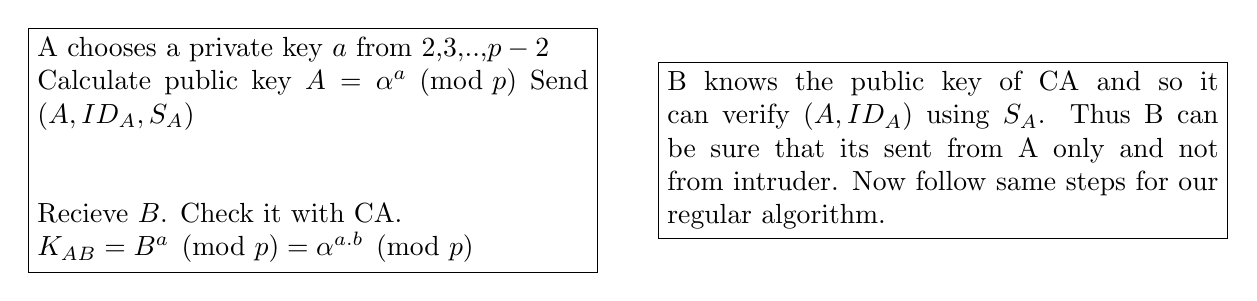
\begin{tikzpicture}
    % First set of text and boxes
    \node[draw, rectangle, minimum width=5cm, minimum height=1cm,anchor=east] (A) at (0,0) {
      \begin{minipage}{7cm}
        A chooses a private key $a$ from {2,3,..,$p-2$} \\
        Calculate public key $A = \alpha^a \pmod{p}$
        Send $(A,ID_A, S_A)$ \\ \\ \\
        Recieve $B$. Check it with CA.\\
        $K_{AB} = B^{a} \pmod{p} = \alpha^{a.b} \pmod{p}$
      \end{minipage}
    };
    \node[draw, rectangle, minimum width=5cm, minimum height=1cm,anchor=east] (B) at (8,0) {
      \begin{minipage}{7cm}
        B knows the public key of CA and so it can verify $(A,ID_A)$ using $S_A$. Thus B can be sure that its sent from A only and not from intruder.
        Now follow same steps for our regular algorithm.
      \end{minipage}
    };

    % \draw[->, thick] (7,-4) -- (10, -7);
    % \draw[->, thick] (10, -4) -- (7,-7);

\end{tikzpicture}

\centering   
\end{figure}

Now, if intruder wants to do something, it can't give fake signature of CA about $A=\alpha^a \pmod{p}$ and ID as private key of CA is not known to anyone. Of cource if CA's private key is known, he/she can break anything on their way. Assuming its not possible, now communication is assumed secure.

\clearpage% Lecture 13 on 7 - 03 - 2024
\noindent\tbox{13}{
\begin{center}  
    \huge Lecture - 13 \\
    \Large Topic: Security Services
\end{center}
}

\section*{Security Services}
\begin{itemize}
  \item Confidentiality
  \item Authentication
  \item Integrity (Not tampered by third party)
  \item Non-repudiation
  \item Access Control
  \item ...
\end{itemize}

Confidentiality can be ensured by Encryption.\\
Authentication can be ensured by Digital Signatures.\\
Integrity can be ensured by Diffusion.\\
Non-repudiation can be prevented by Digital Signatures.\\
\\
Access Control is our next topic of discussion :)
\\
\section*{Elgamal}
Vulnerable to Man in the Middle Attack.\\ 
Solution to this? Certification Authority as we saw in last class.\\
The signature of CA is obtained by providing Public key A and ID\textsubscript{A}. Third party cannot obtain the certification in the name of A as their identity is verified at multiple levels like Govt ID, emails, phonecalls, etc.
Also, the certification comes with a validity period, and should be renewed after that period. Nowadays, the certificate comes along with the device when it is bought.
\\
There is no one centralised CA. The main CA is divided into multiple sub CAs. This is done as if the centralised CA is compromised, then all the data in the world is at risk.
\\
This kind of security is used in SSL, TSL Protocols.\\
SSL - Secure socket Layer \\
TLS - Transport layer security
\\
We have four levels of security:
\begin{itemize}
  \item Application
  \item Transportation Layer
  \item Network Layer
  \item DLL
  \item Physical Layer
\end{itemize}

\clearpage% Lecture 13 on 7 - 03 - 2024
\noindent\tbox{14}{
\begin{center}  
    \huge Lecture - 14 \\
    \Large Topic: Security Protocols(Guest Lecture)
\end{center}
}
\\
Have you ever noticed broken lock symbol in unsafe websites? What are these? How do we actually send messages?
\section*{Digital certificate}
Every device would have a digital certificate which contains information like the person's identity(eg- name, address, organisation), public key, some serial number, validaity dates, certification authority's identity, its digital signature, etc which would be verified by the CA(Certificatation Authority). So indirectly, every user trusts the CA (or whoever is the issuer of the certificate).
All the personal information would be stored in a data stucture, and certificate would be issued by it. But CA cannot certify all over the world right? Traffic would grow exponentially. So, CA can also allot people, and give a certificate that, this firm can issue certification. So end users can believe certificate issued by either CA, or by firms approved by CA. Actually, we can choose organisations that we trust for certification issuing. Many organisations, banks do this.
Try this at room using the slides.

\section*{Protocol against Middle Man Attack}
Say person Alpha wants to send message to Beta and there is a middle man Gamma trying to decrypt it. Each have a certificate from CA for their public key. With the public key of the CA, anyone can verify the certificate. Now, everyone knows everyone's public key, their cerificates. So if Alpha wants to send to Beta, he can use Beta's public key so that only Beta can decrypt it.
When we make connection with google with https, we authenticate google using its certificate. See the slides, for SSL protocol where exchange of messages to google is clearly mentioned.

This is a broadcast system where each person can see anyone's message transaction with everyone having certificate and public keys. But, can an internet service provider(ISP like Jio/ Airtel) interfere in between? Actually, every internet packet is through ISP only, and so they can do anything they want.
SSL certificates are for websites mainly. For emails, its seperate, for whatsapp, or facebook, it different it seems.

\clearpage% Lecture 13 on 7 - 03 - 2024
\noindent\tbox{15}{
\begin{center}  
    \huge Lecture - 15 \\
    \Large Topic: Security Protocols(Guest Lecture)
\end{center}
}

\section*{Revoking a certificate}
Say you have your physical id card. And the institute wants to revoke it before the day of expiry. Since its physical, it can be broken, and revoked, but how to invalidate a digital certificate. We can't delete the certificate simply as its known by everyone. Also, if a person is offline, he won't Recieve the info that its revoked. We can't maintain a revocation list as there might be many certificates revoked everywhere, and its very difficult.
There is a heirarchy of certification agencies which makes it more difficult. 

\section*{Replay Attack}
Say a car is unlocked by a key with IR transmitter. It can be listened, and replayed, or re created to unlock the car. This kind of attack is called replay attack. To avoid this, we can include time stamp along with the message.
\\
\\
So, see both the problems mentioned above. A certificate comes along with a freshness term to represent a time stamp at which a certificate is created.

\section*{Authorization / Access Control}
We have seen before what both means. We need to somehow maintain permissions for each person to view/edit any data.
There are two types of Access control:
\begin{itemize}
  \item[DAC:] Discresionary access control.\\ The owner has the full control over who can read the file, who can update/modify, etc.
  \item[MAC:] Mandatory access control. \\ Irrespective of who is the owner, the sytem administrator has to enforce in system level. He need to design a policy and needs a mechanism to enforce it.
  There would be system, and people with an account in it can login on it. Based on his username or something, the system administrator should enforce that for that user, some of the files are available.
\end{itemize}

\section*{Subject(principle),Object(resources),Action}

Matrix:
Here we have a matrix with columns as objects, and rows as subjects(users). The matrix simply indicates the permission each user has over the files(objects).

% DRAW THE MATRIX

Suppose user 2 wants to read file 3, the matrix says only write, so he cant read file 3. This Matrix is simply to maintain access control. \\ 
This is not an efficient way of maintaining access control - \textbf{Sir} \\

A more systematic way to maintain these permissions is by creating an access control list, for each file s list of the permissions each user have on it.
The list can also be maintained capability wise, that is a list of permissions of particular user one every file. \\

\subsection*{Confused deputy problem}
A compiler has read for

\subsubsection*{solution}
Capability-wise list is safer because ... hmm... not sure 

\clearpage% Lecture 13 on 7 - 03 - 2024
\noindent\tbox{16}{
\begin{center}  
    \huge Lecture - 16 \\
    \Large Topic: DAC and MAC
\end{center}
}

\section*{ACM(access control matrix)}
This we have seen last class that permissions of every file and every user are stored in a matrix.

\section*{ACL(Access control list)}
This is a big list which 

\section*{Confidentiality bases access control model}
Some of such models are:
\subsection*{Bella La Pudela model(BLP)}
So we have subjects(users) $S$, and objects(files) $O$. Now, we have different levels of secracy of an object. They are - top secret, secret, confidential, and unclassified(public). Eg- some persons email is confidential, asc report is secret, and some other very important thing is top secret.
These 4 categoried can be given to the objects. Then we assign a clearence label of a particular subject i.e, what all level files can he/she wants. Now, if a person has clearence level of top secret, then he littrally can see any resources they want. Coming down the heirarchy, the resources will be limited.
This kind of policy is called ``NO READS UP'', i.e a person can't read files of higher sensitive information than their clearence level. Here, for writing, we follow something called ``NO WRITES UP'' where you can't write files of lower priveldge level. Thus, here, even though a public writes on a secret file, it won't be able to be read by other public people.
Thus confidentiality is maintained. This may seem stupid as a public person has access to change secret info. But here, we don't care about other things, and we only care about confidentiality.

\subsection*{Integrity}
In the previous method, we just implement ``NO WRITES UP'' and ``NO READS DOWN''. This can be observed to ensure integrity, i.e, un-authorised people can't write on secret files.

\clearpage% Lecture 13 on 7 - 03 - 2024
\noindent\tbox{18}{
\begin{center}  
    \huge Lecture - 18 \\
    \Large Topic: DAC and MAC
\end{center}
}

Previous class we discussed about information flow. There, we imagine a machine giving output according to input, and knowing the output, will we be able to find the inputs or not was the question.

\section*{Lattice based information flow model}
Here, there is a direction of information flow, and based on whether its legitimate or not, etc, we can model it as a latice. We construct a partial order where the directed edges indicates the legitimate flow of information. Eg, if $x \le y$, then its legitimate if information flow happens from $x$ to $y$.
\begin{figure}[h!]
  \centering
  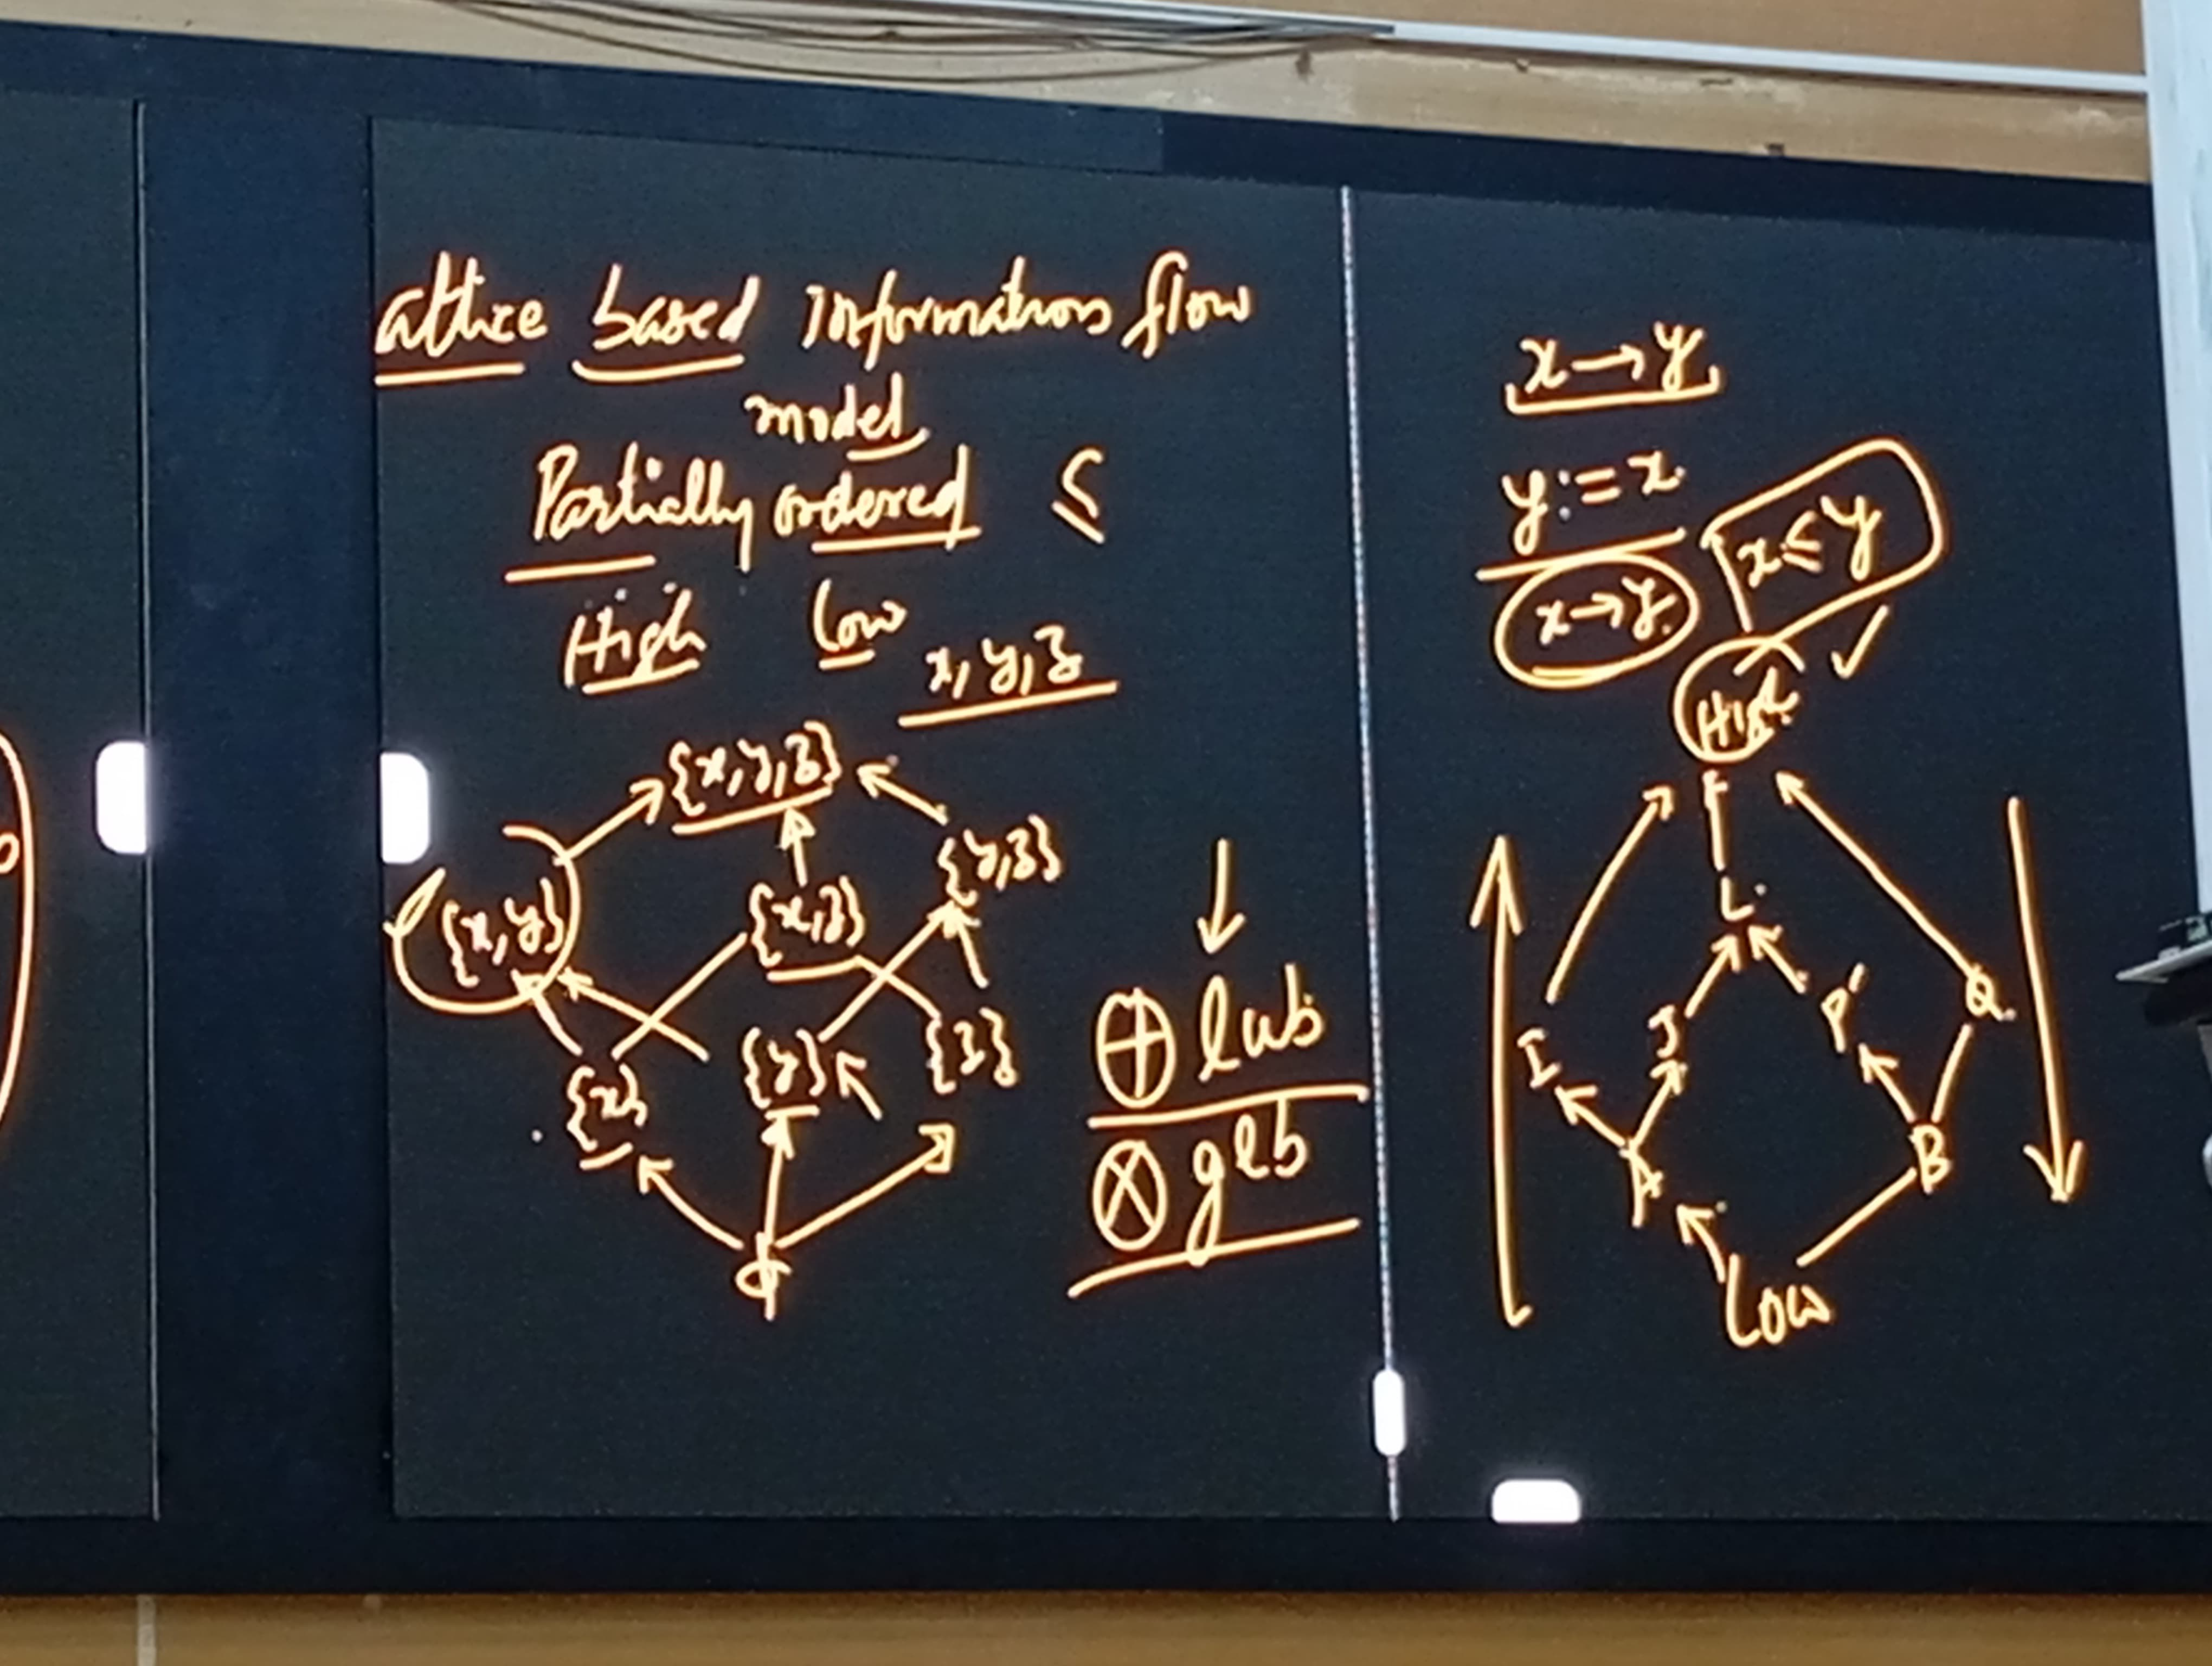
\includegraphics[width=0.8\textwidth]{images/partial_order.jpg}
  \caption*{Partial order}
\end{figure}
We define two operators in latice, namely lowest upper bound ($\oplus$), and greatest lower bound ($\oplus$).

\subsection*{Example}
Say we write $y = x+z, p = y + t$, so there is a info flow from $x \rightarrow y(x \le y)$, $z \rightarrow y(z \le y)$ but, there is no info flow from $y \rightarrow p$ \footnote{This is because, there would have been a value of y which we know, but after its over written by $x$ and $z$. So now using $p$, we can infer only about the new value, and not the previous one.}.

Some of the properties of this model are :-
\begin{enumerate}
  \item reflexive ($A \le A$)
  \item transitive. If info flows from A to B, and B to C, we can say it flows from A to C.
  \item Anti-Symmetric. If info flows from A to B, and B to A, only possibility is that $A = B$.
\end{enumerate}

\section*{RWFM}
Its read write flow model.

\section*{Information Leaking}
What if the algorithm is correct, but its implemented wrongly which leads to information leakage. This is called a Bug. We can identify this by methods like Static Analysis. We can dry run(i.e, mentally run it and see for implementation bugs) the code.

\clearpage% Lecture 13 on 7 - 03 - 2024
\noindent\tbox{18}{
\begin{center}  
    \huge Lecture - -- \\
    \Large Topic: Mid sem solutions
\end{center}
}

\begin{enumerate}
  \item \begin{enumerate}
          \item integrity
          \item availability, confidentiality
          \item integrity / confidentiality
          \item availability, confidentiality
        \end{enumerate}
  \item 21 bits
\end{enumerate}

\clearpage% Lecture 13 on 7 - 03 - 2024
\noindent\tbox{20}{
\begin{center}  
    \huge Lecture - 20 \\
    \Large Topic: Browser Security
\end{center}
}

Mostly, whatever website you login to, its asks for either its own login, or authentication, or google's account, etc. So, we believe google, facebook to keep our login passwords safely, and so we get in through google credentials. So now, what is the conversation, or policy between google and that particular website?

Google gives an API, and whichever website uses it, google lends its authentication to it. Also here, google is a witness for your activites in the website. It actually, now can see how many times you logged in, etc and so it can give suggestions accordingly.

\section*{Cookies}
Its a mechanism to not ask the user again and again for our preferences. Eg- if you choose your preferred language, it'll be stored in cookie, and the next time you login, it knows the preference. Cookie, is a file, stored in a browser side to store such things. It may also contain your passwords. So is it possible for it to get stolen?
\begin{itemize}
  \item If we use a shared computer, since the cookie is stored in the computer only, if another user uses it, it can get leaked.
\end{itemize}
Cookies are encrypted today to avoid the stealing.

Though they are encrypted, there are some ways to break it. They are
\subsection*{XSS(cross site scripting)}
its a type of computer vulnerability typically executed with the help of web applications through breaches in user's web browser. Eg- if some website takes input, you can input a javascript code which modifies the javascript of the website and thus crashing it.

\begin{figure}[h!]
  \centering
  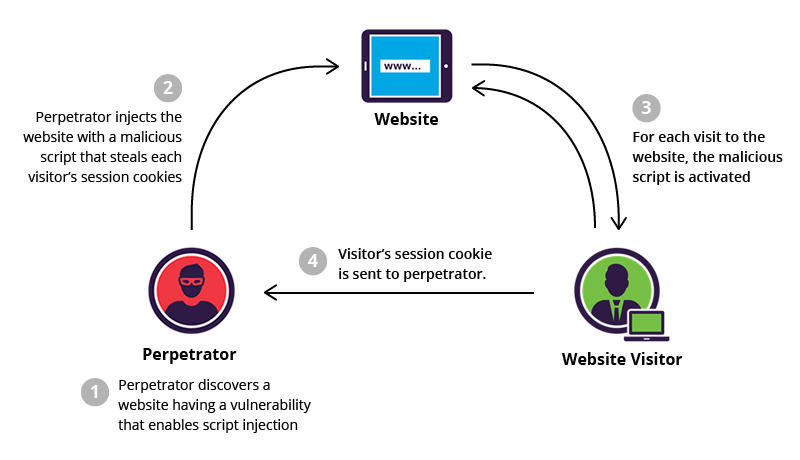
\includegraphics[width=0.75\linewidth]{images/XSS.png}
\end{figure}
To avoid this, if we see some script like input, we ignore it. Nowadays, most websited so this, but an unaware web developer could be a harm for its user.

\subsection*{Reflected XSS}
There are two methods of providing the input to the website. They are GET and POST methods.

In GET method, the information is directly given in the url and the web's code reads from the url and takes it as input and run accordingly. Eg- instead of searching for the string ``data security''  in google's tab, you can direcly give the url you're seaching for itself as \href{https://www.google.com/search?q=data+security}{https://www.google.com/search?q=data+security}.

So, in this method, lets say a hacker gives you a link with input as a javascript, then if you click on it, the website starts working accoding to the hacker's contol.

\subsection*{CSRF}
Typical practical scenario will be like, if you login in some website though your username, pwd, etc and you log out, the session should expire and authentication should end. But if csrf is not handled properly and you click back button, from your history, you can see again your personal data in website even after logging out.

\clearpage% Lecture 13 on 7 - 03 - 2024
\noindent\tbox{21}{
\begin{center}  
    \huge Lecture - 21 \\
    \Large Control Flow
\end{center}
}

\begin{itemize}
  \item Control Flow Integrity Check (CFI)
  \item Malware Detection
  \item Side Channel Based Attacks
\end{itemize}

\section*{Malware Detection}
Signatures

\section*{Behaviour}
Behaviour of a program is .

\section*{Side Channel Based Attacks}
Ciphers used today are vulnerable after quantum computers. Post Quantum Cryptography is lattice based cryptography. \\
Hardware is designed to offer maximum performance while consuming minimal power. Earlier performance was the primary goal, but these days it is minimal power consumption. \\

% \begin{figure}[h!]
%   \centering
%   \includegraphics[width=0.8\textwidth]{ss.jpg}
%   \caption*{Partial order}
% \end{figure}

Performance increase per year vs time \\
\begin{itemize}
  \item 20\% /year - before 1985/86 
  \item 50\% /year - 1985 - 2003/2004 (motto : faster is better) 
  \item 20\% /year - after 2003 (motto : more is better) 
\end{itemize}

But memory accesses are significantly slow (about 100 times slower) which grew at about 6\%/year. Caches were introduced to enhance memory access.
\\
It was believed Control flow was the bottleneck. 
Actually, while a program runs, 10\% of the code executes for 90\% time. 
This can be prevented by speculating and predicting the direction after a conditional. \\

Once the control flow is fixed, data flow became the bottle neck.

\section*{Various performance enhancements:}
\begin{itemize}
  \item Speculation of branch direction.
  \item Speculation of Data.
  \item Out of order execution.
  \item Use of Caches.
  \item Multithreaded architecture support.
\end{itemize}

\clearpage% Lecture 13 on 7 - 03 - 2024
\noindent\tbox{22}{
\begin{center}  
    \huge Lecture - 22 \\
    \Large Topic: Malwares
\end{center}
}

Since every laptop nowadays are connected to internet, malware is common to occur. It means the ability to sneak in another person's system.
Malicious code is a code aimed to harm a system's usage or the user.
Categories:
\begin{itemize}
  \item Virus
  \item Worm
  \item Backdoor
  \item Trojans - spying and entering a system with some other identity. Almost 70\% of the malware attacks are trojans only.
\end{itemize}

There is a requirement to avoid these as these attacks may be as costly as billions of USD. From the past malware attack data, we observe that though number of such attacks are growing exponentially, the total number of distict families of attacks grow only linealy with time. This is a good news that we just need to prevent attacks of a family.

Phishing is another common attack where spam emails are sent to steal login credentials of users.

\section*{Modelling Malware}
A computer virus is a program that can infect ... - a formal defenition was given(refer to slides).
\paragraph*{}
Possibility of a virus infection is based on the theory of self-reproducing automata and not based on system damage or anything.

\begin{theorem}
  For every defence mechanism, there exists a virus that escapes it and for every virus, there exists a defence mechanism for it.
\end{theorem}

Key defenitions:
\begin{itemize}
  \item family- all viruses having a same code base belong to same family
  \item variant- virusus which are just slightly modified from others.
\end{itemize}

\section*{Methods to prevent virus}
Using signatures for programs. We can allow only programs of known signature to run and not run otherwise. The problem with this is that the number of virus is also so much and checking them one by one would be a very difficult job.
In fact, virus detectors like McFree, etc have a full database of signatures of viruses and it checks regularly.

A better option would be to detect malware families and not individual instances. If you see for individual instances is that, if you just add a ``no operation statement'' in your code, the signature, file size, and everything would change though the behaviour would be exactly the same.

To detect code pattens, AI could be used which learnt already existing virus's code bases, and identify the new variant viruses.

\clearpage% Lecture 13 on 7 - 03 - 2024
\noindent\tbox{23}{
\begin{center}  
    \huge Lecture - 23 \\
    \Large Topic: Slides revision in moodle
\end{center}
}

\begin{itemize}
  \item[Trust anchor: ] The root of CA is completely trusted to be true, and its trust cannot be derived. It is assumed to be genuine.
  \item[UI/UX symbols: ] if its green, its secure. If it reads ``not secure!'' in grey, then it means it was once trusted, and maybe the certificate has expired. ``not secure'' in red means it was never trusted.
  \item[Wildcard DC: ] Wildcard Digital certificate is given for a whole domain rather than individual websites. Eg- if ``*iitb.ac.in'' is verified, anyone having website in that domain is verified.
  \item[Types: ] Certificate pinning or stapling- Some certificates are hardcoded and cannot be revoked. Eg - hardware devices, Proof carrying code, some mobile apps, etc.
  \item[] 
\end{itemize}

\section*{CRL (Certificate Revocation List)}
A CRL will list all the certificates that have been either suspended or revoked. CRLs are published by Certificate Authorities. Generally, the root certificate for a Certificate Authority will specify the location of that CA's CRL.

\section*{OCSP (Online Certificate Status Protocol)}
As you login to a website, first we need to check its authenticity with the CA. Checking this can be done is OCSP protocol.
OCSP Stapling improves performance by positioning a digitally-signed and time-stamped version of the OCSP response directly on the webserver.  This stapled OCSP response is then refreshed at predefined intervals set by the CA.  The stapled OCSP response allows the web server to include the OCSP response within the initial SSL handshake, without the need for the user to make a separate external connection to the CA.
OCSP (Online Certificate Status Protocol) is one of two common schemes used to maintain the security.
\\ \\
If the server's certificate returns true upon OCSP (Online Certificate Status Protocol) check,
it means that the certificate is valid according to the issuing Certificate Authority (CA). The termination of the protocol would typically occur during the SSL/TLS handshake process, specifically during the Certificate Verification step.
During the SSL/TLS handshake, after the client receives the server's certificate, it performs a series of checks to verify the certificate's authenticity, including checking the certificate's expiration date, verifying the signature, and optionally checking the certificate's revocation status using OCSP or Certificate Revocation Lists (CRLs). If the OCSP check returns true, indicating that the certificate has not been revoked, the certificate is considered valid, and the handshake can proceed.

OCSP is usually used in transactions where the validity of digital certificates needs to be verified in real-time. This is particularly important in situations where immediate assurance of a certificate's validity is required, such as in online banking, e-commerce transactions, secure email communication, and accessing secure websites (HTTPS). By checking the certificate's status via OCSP, parties involved in the transaction can ensure that the certificate has not been revoked since it was issued, thereby enhancing the security of the communication channel.

\section*{Perspectives}
Perspectives is a decentralized approach to securely identifying Internet
servers. 
Network notaries are like CAs found across the internet and carry the digital ceritficates of various websites. Once a user accesses a website the browser verifies the digital certificate of the website and compares it with the previous certificates tracked by the trusted network notaries. If they differ then we know there is a Man in the Middle attack.

\section*{Certificate Pinning by OS/Browser}
Explanation: Certificate pinning is a security mechanism used by web browsers, operating systems, and applications to prevent man-in-the-middle attacks and certificate spoofing. By pinning (or associating) a website's digital certificate with its public key or cryptographic hash, the browser or OS can ensure that subsequent connections to the website only accept certificates signed by the pinned key. This helps protect against attacks where an attacker presents a fraudulent certificate signed by a compromised or rogue CA.

\end{document}